\documentclass{report}
%change the margins
\usepackage[margin=1in]{geometry} 
% used for adding todo notes
\usepackage{todonotes}
% Used for adding Matlab Algorithms
\usepackage{listings}
\usepackage[framed,numbered]{matlab-prettifier}
%Adds link to script
\usepackage[hidelinks]{hyperref}
%use fo rdefining new column
\usepackage{array}
%Add urls
\usepackage{url}
%use for numbered lists
\usepackage{enumerate}
% Add images
\usepackage{graphicx}
%lets you use the [H] command to force float placement
\usepackage{float}
%table toprule, midrule, bottomrule
\usepackage{booktabs}
%Use for folder tree
\usepackage{xcolor}
\usepackage{dirtree}
%multirow in tables
\usepackage{multirow}
%degree symbol
\usepackage{gensymb}
%align equations
\usepackage{amsmath}
%checklist
\usepackage[ampersand]{easylist}
%pros/cons list
\usepackage{booktabs}
\usepackage{tabularx}

% Change name from listing to algorithm
\renewcommand{\lstlistingname}{Algorithm}% Listing -> Algorithm
\renewcommand{\lstlistlistingname}{List of \lstlistingname s}% List of 
%make references include the type of reference
\newcommand*{\tabref}[1]{\tablename~\ref{#1}}
\newcommand*{\figref}[1]{\figurename~\ref{#1}}
\newcommand*{\algref}[1]{\lstlistingname~\ref{#1}}
\newcommand*{\eqnref}[1]{Equation~\ref{#1}}
\newcolumntype{C}[1]{>{\centering}m{#1}}
\newcommand{\treeDB}[1]{  \includegraphics[scale = 0.3]{../figures/icons/DatabaseProject.png}\ {#1}}
\newcommand{\treeFolder}[1]{  \includegraphics[scale = 0.3]{../figures/icons/folder.png}\ {#1}}
\newcommand{\treeMatlabM}[1]{  \includegraphics[scale = 0.3]{../figures/icons/m.png}\ {#1}}
\newcommand{\treePhotoscanFolder}[1]{\includegraphics[scale = 0.3]{../figures/icons/photoscandocx.png}\ {#1}}
\newcommand{\treeTxt}[1]{  \includegraphics[scale = 0.3]{../figures/icons/text-document.png}\ {#1}}
\newcommand{\treeImg}[1]{  \includegraphics[scale = 0.3]{../figures/icons/pictures.png}\ {#1}}
\newcommand{\treeGopro}[1]{  \includegraphics[scale = 0.3]{../figures/icons/device.png}\ {#1}}
\newcommand{\treeLAS}[1]{  \includegraphics[scale = 0.3]{../figures/icons/cc.jpg}\ {#1}}
\newcommand{\treePPT}[1]{  \includegraphics[scale = 0.3]{../figures/icons/ppt.png}\ {#1}}
\newcommand{\treeArduino}[1]{  \includegraphics[scale = 0.3]{../figures/icons/Arduino.png}\ {#1}}
\newcommand{\treeXLS}[1]{  \includegraphics[scale = 0.3]{../figures/icons/excel.png}\ {#1}}
\begin{document}
	\begin{titlepage}

\newcommand{\HRule}{\rule{\linewidth}{0.5mm}} % Defines a new command for the horizontal lines, change thickness here

\center % Center everything on the page
%----------------------------------------------------------------------------------------
%	LOGO SECTION
%----------------------------------------------------------------------------------------


\includegraphics[width = 2.5in]{../figures/birdword.png}\\[1cm] % Include a department/university logo - this will require the graphicx package
 
%----------------------------------------------------------------------------------------
%	HEADING SECTIONS
%----------------------------------------------------------------------------------------

%\textsc{\LARGE Cormorant Analytics}\\[1.5cm] % Name of your university/college
\textsc{\large }\\[0.5cm] % Major heading such as course name
\textsc{\large }\\[0.5cm] % Minor heading such as course title

%----------------------------------------------------------------------------------------
%	TITLE SECTION
%----------------------------------------------------------------------------------------

\HRule \\[0.4cm]
{ \huge \bfseries Final Report}\\[0.4cm] % Title of your document
\HRule \\[1.5cm]
 
%----------------------------------------------------------------------------------------
%	AUTHOR SECTION
%----------------------------------------------------------------------------------------

%\begin{minipage}{0.4\textwidth}
%\begin{flushleft} \large
%\emph{Authors:}\\
%Richard \textsc{Slocum} \\ % Your name\\
%Kory \textsc{Kellum} % Your name\\
%\end{flushleft}
%\end{minipage}
%~
%\begin{minipage}{0.4\textwidth}
%\begin{flushright} \large
%\emph{Professor:} \\
%Dr. Mike \textsc{Olsen}\\% Supervisor's Name
%\ 
%\end{flushright}
%\end{minipage}\\[4cm]

% If you don't want a supervisor, uncomment the two lines below and remove the section above
\Large \emph{Prepared By:}\\
Richard \textsc{Slocum}\\[7cm] % Your name

%----------------------------------------------------------------------------------------
%	DATE SECTION
%----------------------------------------------------------------------------------------

{\large March 10, 2016}\\[3cm] % Date, change the \today to a set date if you want to be precise


 
%----------------------------------------------------------------------------------------

\vfill % Fill the rest of the page with whitespace

\end{titlepage}
	\cleardoublepage
	\pagenumbering{roman}
	\chapter*{Introduction}
		Cormorant Analytics improved upon a previous Multi-View Stereo Sensor by implementing a new prototype system consisting of new camera hardware, triggering electronics, 3D printed mount and enclosures, and Matlab processing algorithms.  The sensor was successfully integrated on a 3D Robotics X8 Quadcopter UAS platform.  A camera layout was selected to optimize the field of view of the sensor for long timeseries data acquisition of breaking waves in the littoral zone.  Camera boresight and relative orientation between the cameras is calculated and reported using the CAD model.  The system was succesfully integrated onto a 3D Robotics X8 Octocopter for initial testing.
	Cormorant Analytics also provided support for processing previously acquired imagery through Agisoft Photoscan, as well as generation of Orthophotos with previously developed algorithms.  All of the Delivery Milestones, outlined in \tabref{tab:milestone}, were completed on time.
	\begin{table}[htbp]
		\centering
		\caption{All Milestones were completed on time.}
		\begin{tabular}{rrr}
			\toprule
			\textbf{Delivery Order Milestones} & \multicolumn{1}{c}{\textbf{Scheduled Completion}} & \textbf{Actual Completion} \\
			\midrule
			Project Kick-Off Meeting & 15-Mar & 15-Mar \\
			Quarterly Program Management Review & 15-Jun & 15-Jun \\
			Quarterly Program Management Review  & 15-Sep & 15-Sep \\
			Initial Prototype Delivery & 15-Oct & 15-Oct \\
			Quarterly Program Management Review & 15-Dec & 15-Dec \\
			Close-out Brief & 15-Mar & 15-Mar \\
			\bottomrule
		\end{tabular}%
		\label{tab:milestone}%
	\end{table}%
%	\cleardoublepage
	\vspace{-1em}
	\section*{Overview of Report}
	\subsection*{Chapter 1: Camera Hardware}
	The decision to use GoPro cameras, as well as the alternative camera options considered are discussed.  The lens and camera orientation are also discussed.
	\vspace{-.2em}
	\subsection*{Chapter 2: Electronics}
	The electronic components, schematic, board, and methodology for triggering via teh GoPro audio port are discussed.  The cable pinout for each cable is also documented and discussed.
	\vspace{-.2em}
	\subsection*{Chapter 3: Mount Design and Fabrication}
	Each component for the sensor design is briefly discussed, as well as the calculation of the relative orientations of the cameras from the CAD model.  
	\vspace{-.2em}
	\subsection*{Chapter 4: Image Synchronization}
	The methodology and algorithms used to synchronize the video files to UTC time is discussed.  Documentation for how to extract images with interpolated GPS position info is also discussed.
	\vspace{-.2em}
	\subsection*{Chapter 5: Acquisition and Data Storage}
	A workflow and checklist for data acquisition is presented.


	\cleardoublepage
	\pagenumbering{arabic}
	\tableofcontents
	\thispagestyle{empty}
	\cleardoublepage
	\setcounter{page}{1}
	

	\chapter{Camera Hardware}
		The previous version of the MVSS sensor could only attain a maximum synchronized frame rate of 0.5Hz, which is inadequate for celerity based bathymetry inversions.  Alternative sensors were assessed and considered, with cost and weight being the major limitations.  After consideration, an array of GoPro Hero 4 Black sensors with modified lenses were selected as the camera sensors. 
	\section{Camera Selection}
	\subsection{GoPro Hero 4 Black}
	GoPro cameras are a Commercial Off The Shelf(COTS) camera that is used by consumers across the world for video and imagery.  While the GoPro sensors have a number of negatives, outlined in the advantages and disadvantages list in \tabref{tab:gopro}, they were ultimately selected due to the low weight, low cost, low power, availability for purchase, and ruggedness of the cameras.
	
	\begin{table}[H]
		\begin{tabularx}{\linewidth}{>{\parskip1ex}X@{\kern4\tabcolsep}>{\parskip1ex}X}
			\toprule
			\hfil\bfseries Advantages
			&
			\hfil\bfseries Disadvantages
			\\\cmidrule(r{3\tabcolsep}){1-1}\cmidrule(l{-\tabcolsep}){2-2}
			Inexpensive\par
			Lightweight\par
			Easy to purchase\par
			Rugged\par
			Low Power Requirements
			&
			CMOS rolling shutter (nonlinear image distortion)\par
			No documented method for time synchronization\par
			High lens distortion 
			\\\bottomrule
		\end{tabularx}
		\caption{Advantages and disadvantages of using GoPro cameras for use in the second version of the MVSS.}
		\label{tab:gopro}
	\end{table}
	
	\subsection{PtGrey}
	PtGrey is an industrial camera manufacturer that manufacturers a wide array of products which contain hardware triggering.  While the hardware triggering of these sensors would be a much more robust and accurate time synchronization methodology, the weight and power requirements were too great for integration on a small Unmanned Aerial System.  The PtGrey Ladybug was also considered, but the weight and power for it made integration on a UAS prohibitive. An advantages and disadvantages list for the PtGrey cameras is shown in \tabref{tab:PtGrey}.
	
	\begin{table}[H]
		\begin{tabularx}{\linewidth}{>{\parskip1ex}X@{\kern4\tabcolsep}>{\parskip1ex}X}
			\toprule
			\hfil\bfseries Advantages
			&
			\hfil\bfseries Disadvantages
			\\\cmidrule(r{3\tabcolsep}){1-1}\cmidrule(l{-\tabcolsep}){2-2}
			Hardware triggering\par
			Well documented API\par
			Reliable\par
			Many Lens Options\par
			&
			Too heavy with lenses and CPU\par
			Requires external CPU for triggering and data storage\par
			Requires a lot of power to run the camera and CPU
			\\\bottomrule
		\end{tabularx}
		\caption{Advantages and disadvantages of using PtGrey cameras for use in the second version of the MVSS.}
		\label{tab:PtGrey}
	\end{table}
	
	\subsection{Raspberry Pi Camera Module}
	Raspberry Pi is an inexpensive, consumer grade linux computer that is marketed towards students and hobbyists.  The Raspberry Pi computer interfaces with a small Raspberry Pi camera module, which can then be used to acquire imagery and video.  After experimenting with the camera, it was determined that the software triggering accuracy of the camera was inadequate for time synchronization across an array of cameras.  The other advantages and disadvantages are shown in \tabref{tab:raspi}.
	
	\begin{table}[H]
		\begin{tabularx}{\linewidth}{>{\parskip1ex}X@{\kern4\tabcolsep}>{\parskip1ex}X}
			\toprule
			\hfil\bfseries Advantages
			&
			\hfil\bfseries Disadvantages
			\\\cmidrule(r{3\tabcolsep}){1-1}\cmidrule(l{-\tabcolsep}){2-2}
			Inexpensive\par
			Lightweight\par
			&
			Low resolution\par
			Inaccurate software trigger\par
			Relatively ``black box'' camera module\par
			Requires a Raspberry Pi for each camera, adding to the power requirements and weight.
			\\\bottomrule
		\end{tabularx}
		\caption{Advantages and disadvantages of using Raspberry Pi cameras for use in the second version of the MVSS.}
		\label{tab:raspi}
	\end{table}
	
	\subsection{CHDK}
	The Canon Hacker Development Kit(CHDK) is an open source project that modifies the firmware of Canon point and shoot cameras to enable advanced image acquisition.  This was used for the first version of MVSS, but the frame rate was too slow.  CHDK was again investigated to see if any improvements could be made to the frame rate, but it was determined that the frame rate could not be improved past the 0.5Hz.
	
	\begin{table}[H]
		\begin{tabularx}{\linewidth}{>{\parskip1ex}X@{\kern4\tabcolsep}>{\parskip1ex}X}
			\toprule
			\hfil\bfseries Advantages
			&
			\hfil\bfseries Disadvantages
			\\\cmidrule(r{3\tabcolsep}){1-1}\cmidrule(l{-\tabcolsep}){2-2}
			Accurate pseudo hardware trigger\par
			High resolution (16Mp)\par
			Lightweight\par
			Low Power\par
			&
			Frequent Undocumented Bugs\par
			Poor Frame Rate\par 
			Retracting Lens causes unstable lens IO parameters
			\\\bottomrule
		\end{tabularx}
		\caption{Advantages and disadvantages of using CHDK cameras for use in the second version of the MVSS.}
		\label{tab:chdk}
	\end{table}
	
	\section{Lens Selection}
	GoPro cameras are constructed with a 2.92mm lens by default, but there is an undocumented method to open the camera and replace the lens. The stock lens mounts into M12 threading, and the whole threading mechanism can be removed and replaced with a product called a ``SuperMount.''  This mount also has M12 threading, but allows for longer focal lengths to be installed.  There were four lenses on the market that advertised a `High Mp' lens for the M12 threading, and each are compared in \figref{fig:lenscomp}.  The 2.9mm after-market lens was eliminated as an option because it exhibited excessive radial distortion and vignetting.  The default, 4.35mm, and 5.4mm lenses were considered as options when designing the camera orientations.   
	
	\begin{figure}[H]
		\centering
		\includegraphics[scale = 0.3]{../figures/lenscomp.png}
		\caption{The four M12 lenses were tested in the GoPro camera, and it was determined that the 2.9mm lens should not be used due to excessive vignetting and distortion.  The default, 4.35mm, and 5.4mm lenses were considered as options when designing the camera orientations.}
		\label{fig:lenscomp}
	\end{figure}

	\section{Possible Improvements}
	The current GoPro sensor design functions as a prototype, but will likely require debugging and troubleshooting to become a robust sensor for repeated data acquisitions.  The GoPro camera is the greatest limiting factor in the system, and efforts should be made to continue explore more robust, industrial camera options as camera technology progresses.  Future work should continue to monitor the virtual reality camera and cell phone camera markets, as these consumer technologies hold great promise for an improved sensor.  These types of cameras may have time synchronization built in, which is the largest issue with this current system.
	
	\chapter{Electronics}
	Synchronization of the GoPro cameras is essential for seamless orthophoto generation and boresight calculation.  The GoPro cameras do not have any documented methods to synchronize either video or imagery acquired with more than one camera.  A custom solution was developed to utilize the external microphone port of the GoPros in order to embed metadata in any recorded video files.  The approach using the audio port was selected, and is integrated in a modular manner, so that alternative video cameras with an external microphone option can be synchronized in the future using this same methodology.  
\section{Other Considered Methodology}
An alternative approach using a GoPro remote trigger was also investigated, but proved to be inadequate.  GoPro cameras can also be purchased with an external, handheld remote which operates over wifi to trigger one or more cameras.  This approach was investigated and tested for feasibility by triggering four GoPro cameras indoors.  The variable latency between when the remote was pressed and each GoPro began acquiring data was clearly discernable through the audible beep that each camera made when the command was received and acknowledged.  The audible beep variability between cameras was sometimes on the order of tenths of a second, which is far too great of an offset for accurate triggering.  Had the cameras been triggered at the exact same time, further investigation would have still been needed to ensure that there was no temporal drift between cameras. 

\section{Audio Encoding Technical Approach}
The methodology to time sync the imagery relies on the two audio channels (left and right) of the GoPro.  The left channel received the Binary counter integer once a second, and the right channel records the raw PPS from the GPS.  The Teensy microcontroller records the exact time it sent the binary signal to the GoPro.  This establishes a correspondence between the Teensy and GPS time frame.  The GPS also sends the PPS and GPS NMEA string to the Teensy, which can be used to solve for a time synchronized pointcloud to UTC time.

The binary signals sent to the GoPro are timestamped with the GoPro internal time, which is synchronized to the video frames that are being acquired.  These type of binary signals are normally decoded by a serial port, but a custom solution was developed to decode the information from the audio signal.  These signals are then decoded in pos- processing to synchronize the GoPro Video frames to GPS time.  This methodology only works when the GoPros are in video mode, and therefore the spatial resolution is limited compared to the image frame capture capabilities.

An initial approach to record raw NMEA sentences from a GPS receiver was unsuccessful due to difficulties in decoding the raw data, as well as bandwidth limitations.  A theoretical maximum of only 48kbs could be sent over each microphone channel due to the fixed sampling frequency of the GoPro microphone port, however in practice this value is much lower due to signal conditioning.  For this reason, an alternative approach utilizing a SD card for data logging was selected. 

A microcontroller is used as the system master, and it interfaces with a GPS receiver, a SD card logger, and the GoPro external microphone ports.  The microcontroller is constantly recording GPS NMEA data directly to the SD card, and logging it with an internal timestamp depicting when the GPS data was received.  Note that this timestamp certainly has some latency associated with it, as the timestamp is only recorded once the GPS has processed the raw signals and the microcontroller has acknowledged receipt of the serial data.  For this reason, the PPS signal is also recorded to both the SD card and the GoPro external right microphone channel.  This PPS, when coupled with the NMEA string, can provide accurate timestamping with nanosecond precision.  Due to the latency between video frames and audio recorded by the GoPro, as well as the interpolation between frames acquired at 30Hz, nanosecond precision can not be achieved with this methodology.  Further details on the processing of the GoPro audio and Teensy logfile to achieve timestamped video is explained in detail in Chapter \ref{ch:sync}.

\section{Component Selection}
The components for the PCB were selected to minimize space, weight, and power requirements.  The following components were selected and integrated onto the PCB, and a short description of the part is provided.
\subsection{Teensy 3.2}

\url{https://www.pjrc.com/teensy/teensy31.html}\vspace{0.5em}

The Teensy 3.2 microcontroller is a 32bit, breadboard friendly microcontroller that operates on 3.3V logic.  It was selected mainly due to the small form factor and access to the three Serial ports required for interfacing with the SD card, GPS, and GoPro camera.  Compared to Arduino brand microcontrollers with similar capabilities, the Teensy 3.2 is also lower cost and has increased performance.  The Teensy can be programmed with the Arduino IDE, so the transition from Arduino code used in previous iterations of the sensor to the Teensy was seamless.  
\subsection{openLog}

\url{https://www.sparkfun.com/products/9530}\vspace{0.5em}

The openLOG is a lightweight, easy to implement data logger that takes any serial data passed to the RX port and logs it to a microSD card.  The SD card is initially set to a default 9600 baud rate, but the config.txt file on the sd card is modified for this project so that it logs at 115200.  The SD card must have the config.txt file with the baud rate field set to 115200 for the current code to work.
\subsection{Adafruit Ultimate GPS}

\url{https://www.adafruit.com/products/746}\vspace{0.5em}

The Ultimate GPS is a low cost L1 only GPS receiver that has a PPS output.  It was selected because it is low cost, lightweight and easy to integrate as it has the digital io pins broken out to headers.  The PPS pin in conjunction with the NMEA GPS string provides accurate timestamping of the imagery, as well as a low quality GPS position.
\subsection{Voltage Regulator}

\url{https://www.adafruit.com/products/1065}\vspace{0.5em}

The ``Mini DC-DC 5V Stepdown'' regulator was chosen as it provides up to 94\% efficiency and up to 1A output.  It also has a 6.5-32V input range, which allows for various battery options to be explored.  The high efficiency of the DC-DC stepdown enables smaller and lighter batteries to be used.
\subsection{9 Degree of Freedom IMU}

\url{https://www.sparkfun.com/products/13284}\vspace{0.5em}

The LSM9DS1 is a 9 degree of freedom motion sensing chip that houses a triad of accelerometers, gyroscopes, and magnetometers.  This Chip was selected as it is very lightweight, low cost, and should contain the ability to generate low accuracy camera poses.  It communicates via I2C protocol, and therefore an extra serial port is not required.
\subsection{JST Connectors}

\url{https://www.sparkfun.com/products/9916}\vspace{0.5em}

JST connectors are a brand of connector that connects a breadboard to a cable.  These are purchased with the wires already broken out for ease of integration in 2-pin, 3-pin, and 4-pin connector packages.  
\subsection{``SuperBright" LEDs}

\url{https://www.adafruit.com/products/754}\vspace{0.5em}

LED status lights were selected to be as bright as possible because previous data status LEDs were difficult to view in bright, outdoor lighting.  These status lights use more battery, but as they are dubbed "superbright", they are much easier to see.  The polarity of the pins of the LED are important, and are depicted by the length of the wire to the LED.  The longer wire is the positive lead, and the shorter is the negative, as depicted in \figref{fig:led}.  

\begin{figure}[h]
	\centering
	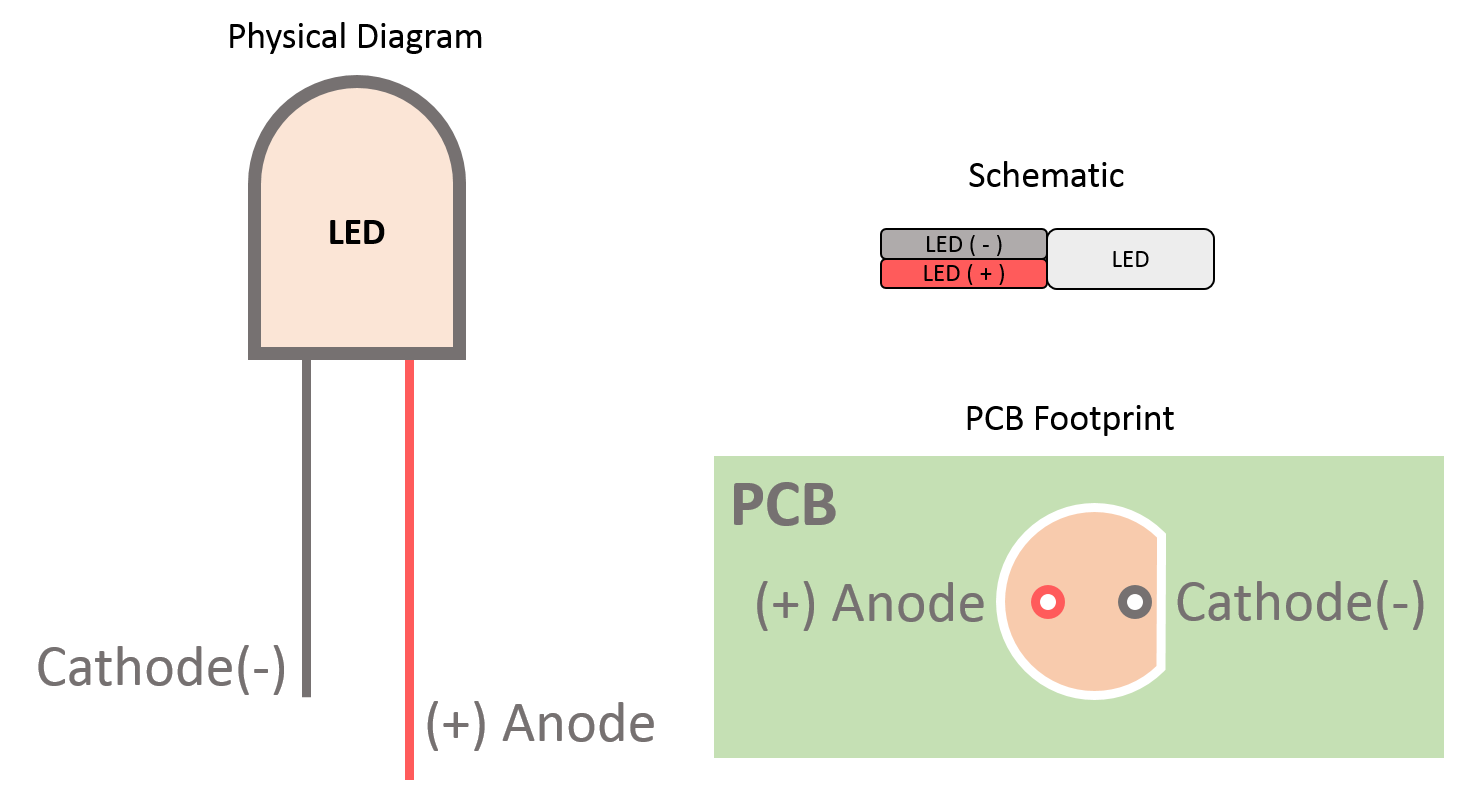
\includegraphics[width = .75\linewidth]{../figures/LED.png}
	\caption{The LEDs used are follow a traditional LED diagram and PCB format, where the longer wire represents the Anode.}
	\label{fig:led}
\end{figure}

\section{PCB Schematics and Board Designs}
EAGLE was used to generate the schematic and board designs for the circuit.  The design was divided into two PCBs.  The first PCB, referred to as the ``Main'' PCB, contains all of the main components of the circuit.  The second PCB, referred to as the ``Panel'' PCB, works as a connector so that the GoPro cables can be connected and disconnected easily from the outside.  
\subsection{Main PCB}
The schematic for the main PCB, shown in \figref{fig:schematic}, is divided into the Power, Voltage Divider, Optional LEDs, Camera Output, Teensy microcontroller and Sensors sections.  Notice that in the Voltage Divider section, in order to ensure the correct Voltage levels into the GoPro microphone port a voltage divider was used to reduce the 3.3V input to approximately 30mV for both the PPS and NMEA ports. 

\begin{figure}[h]
	\centering
	\includegraphics[width = .75\linewidth]{../figures/Schematic.png}
	\caption{The main schematic was designed in EAGLE, and a higher resolution is available in the deliverables folder structure as both a ".sch" and ".png" file.}
	\label{fig:schematic}
\end{figure}

The main board layout, shown in \figref{fig:board}, was designed to minimize the footprint and reduce large cable bending by placing connectors near the edge of the board.  The board was also designed in conjunction with the 3D printed mount, and the shape and orientation was optimized to fit on the electronics tray.  The order that the components are soldered is important such that nothing covers up something that needs to be soldered from the other side of the board.

\begin{figure}[H]
	\centering
	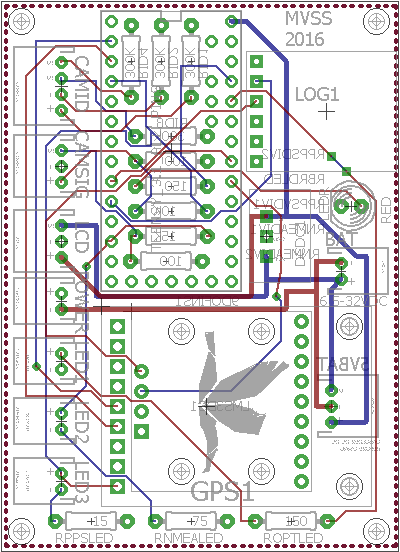
\includegraphics[height = 2in]{../figures/board.png}
	\caption{The main board layout was designed in EAGLE. Red traces represent the top of the board and blue traces represent the bottom.}
	\label{fig:board}
\end{figure}
\subsection{Panel PCB}
The Panel PCB serves as a connection point for the cables that go to the GoPro.  The main PCB outputs the ground signal, two ``pseudo-audio'' signals, and an ``ID'' wire for each camera.  The ground, as well as the PPS and binary ``pseudo-audio'' signals are split into 4 signals each so that the signal can be sent to each of the four cameras.  The ID signals are individually sent to each camera, as the 300k$\Omega$ resistor tying the signal to ground is what tells the goPro to store audio from the ``external audio'' port.  The schematic is shown in \figref{fig:panelschematic}, and the board is shown in \figref{fig:panelboard}.
\begin{figure}[H]
	\centering
	\includegraphics[height = 2in]{../figures/panelZoomschematic.png}
	\caption{The panel schematic was designed in Eagle. This simple PCB is used as a connector so that the 7 signals are split to go to the 16 signals required for the GoPro.}
	\label{fig:panelschematic}
\end{figure}
\begin{figure}[h]
	\centering
	\includegraphics[height = 1in]{../figures/panelboard.png}
	\caption{The panel board layout was designed in EAGLE. Red traces represent the top of the board and blue traces represent the bottom.}
	\label{fig:panelboard}
\end{figure}

\section{Cable Pin Labels}
The pinouts for each of the two PCBs are depicted in \figref{fig:pinouts}.  These cables should be custom made to the correct length so as to reduce the overall weight of the system.  Each of the JST connectors comes with the leads already crimped into the connector and tinned with solder on the other end.  This allows for them to be easily soldered together to generate a solid connection.  
\begin{figure}[H]
	\centering
	\includegraphics[scale = 0.5]{../figures/pinoutmainPCB.pdf}
	\includegraphics[scale = 0.5]{../figures/pinoutpanelPCB.pdf}
	\caption{The pinouts for the main PCB and panel PCB are labeled.  The color of the box represents the color of the wire. }
	\label{fig:pinouts}
\end{figure}

\section{GoPro Mini-USB-B Cable}
The cable that connects the GoPro to the PCB is based on a USB mini-B cable with 10 pins.  It utilizes the pins as shown in \tabref{tab:pinouts}.  The 300k$\Omega$ resistor could have been placed within the cable, or immediately after the socket, as both channel 7 and 3 are right next to each other and a resistor could simple be soldered across the two.  This would reduce the number of wires in the cable from 4 to 3.  However for this version of the cable the resistor is placed on the PCB rather than in the cable to improve the ability to debug the system.  

\begin{table}[h]
	\centering
	\begin{tabular}{l|l}
		\toprule
		Pin Number & Description \\
		\midrule
		Pin 3 & Ground\\
		Pin 4 & Right Audio Channel\\
		Pin 5 & Left Audio Channel\\
		Pin 7 & ID pin which enables the external audio when brought to ground across a 300k$\Omega$ resistor.\\
		\bottomrule
	\end{tabular}
	\caption{The GoPro cable utlizes pins 3,4,5, and 7 to trigger the camera via the audio port.}
	\label{tab:pinouts}
\end{table}

\begin{figure}[H]
	\centering
	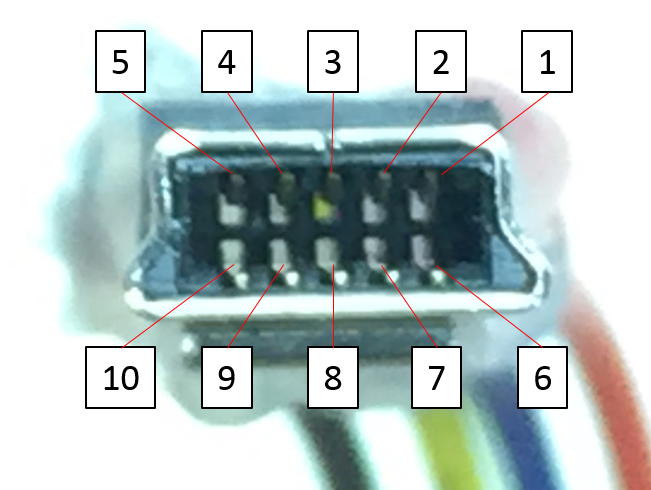
\includegraphics[scale = 0.7]{../figures/tenpin.png}
	\caption{Traditional cables that are purchased in retail stores only break out 4 of the 10 pins in a mini-B connector.  The GoPro triggering cable requires a custom cable, as pins 3,4,5 and 7 are used.}
	\label{fig:pinouts}
\end{figure}

\section{Power}
The power input into the PCB is set up for 6.5V - 32V DC by default, with a maximum output of 1A at 5V.  The average current draw was tested for a 9V battery. The average power draw is calculated using \eqnref{eqn:PVI} shown in \tabref{tab:avgPower}, and estimated runtime calculated with with \eqnref{eqn:estbat} different batteries is shown in \tabref{tab:batRuntime}.
\begin{equation}
\label{eqn:PVI}
Average\hspace{.5em} Power = Voltage \times Current
\end{equation}
\begin{table}[H]
	\centering
	\begin{tabular}{lcr}
		\toprule
		Average Voltage (V) & Average Current (mA) & Average Power (W) \\
		\midrule
		8.3 & 0.080 & 0.664 \\
		\bottomrule
	\end{tabular}
	\caption{The average power draw for the PCB was calculated using a 9V battery.}
	\label{tab:avgPower}
\end{table}

\begin{equation}
\label{eqn:estbat}
Estimated\hspace{.5em}Runtime (hours) = \frac{Battery\hspace{.5em} Voltage \times Battery\hspace{.5em} Current}{Average\hspace{.5em} Power} 
\end{equation}
\begin{table}[H]
	\centering
	\begin{tabular}{lccr}
		\toprule
		Battery Type & Voltage & Estimated Capacity(mah) & Estimated runtime(hours) \\
		\midrule
		9V Battery & 9 & 400 & 5.4\\
		Two 1000mA Lithium Ion & 7.4 & 1000  & 11.1\\
		Three 1000mA Lithium Ion & 11.1 & 1000  & 16.7\\
		\bottomrule
	\end{tabular}
	\caption{The estimated runtime is calculated for a number of potential battery options.}
	\label{tab:batRuntime}
\end{table}
\subsection{Alternate Power}
An alternate method for powering the PCB is provided via a 3-Pin JST connector on the bottom of the board.  The pinout for this port is not documented, as it has not been tested.  The board and schematic should be read to determine the proper power input values.  The connector provides the user access to provide their own regulated 5V battery circuit.  There is one wire for ground, one for 5V, and another for raw voltage.  The raw voltage line is used to monitor battery status and health using the LCD on the front of the panel.

\section{Microcontroller Algorithm}\label{sec:algoLog}
The algorithm to write the logfile to the SD card is programmed using the Arduino IDE.  The Arduino IDE is used as the programming environment for the Teensy, per documentation on the Teensy website.  A flowchart depicting the code is shown in \figref{fig:TeensyFlow}, and the code is provided in electronic form.  Emphasis is placed on ensuring accurate timing, but precedence is placed in this order:
\begin{enumerate}
	\item Accurate retrieval of Teensy time when PPS rising edge is detected
	\item Accurate Teensy time of when counter was sent to gopro
	\item Accurate Teensy time of when the GPS time is received
\end{enumerate}
The three different time references that are used for time syncing are GoPro time, Teensy time, and GPS time.  GoPro time is the internal time of the GoPro camera in seconds from the time the video began recording.  Teensy time is the time in milliseconds since the Teensy was powered on.  GPS time is the Coordinated Universal Time(UTC), which is output from the GPS.  The synchronization between these times is described in more detail in Chapter \ref{ch:sync}, but it is essential that the times are recorded as precisely as possible.  

To ensure that the PPS and Teensy time are accurately correlated, an interrupt routine is implemented in the Teensy algorithm.  An interrupt routine, while technically different than running in parallel, can essentially be seen as a parallel processing task.  In this algorithm, the interrupt is constantly monitoring for the rising edge of the PPS pulse.  When the rising PPS pulse is detected, the code stops whatever it is doing and jumps directly into the interrupt routine.  The interrupt records the exact Teensy time when this occured, and saves it to a global variable before releasing the code to finish performing whatever task it was working on.  It then writes the data to the SD card whenever it is convenient, as once the exact Teensy time is recorded there is no urgency to write the data.  

\begin{figure}[H]
	\centering
	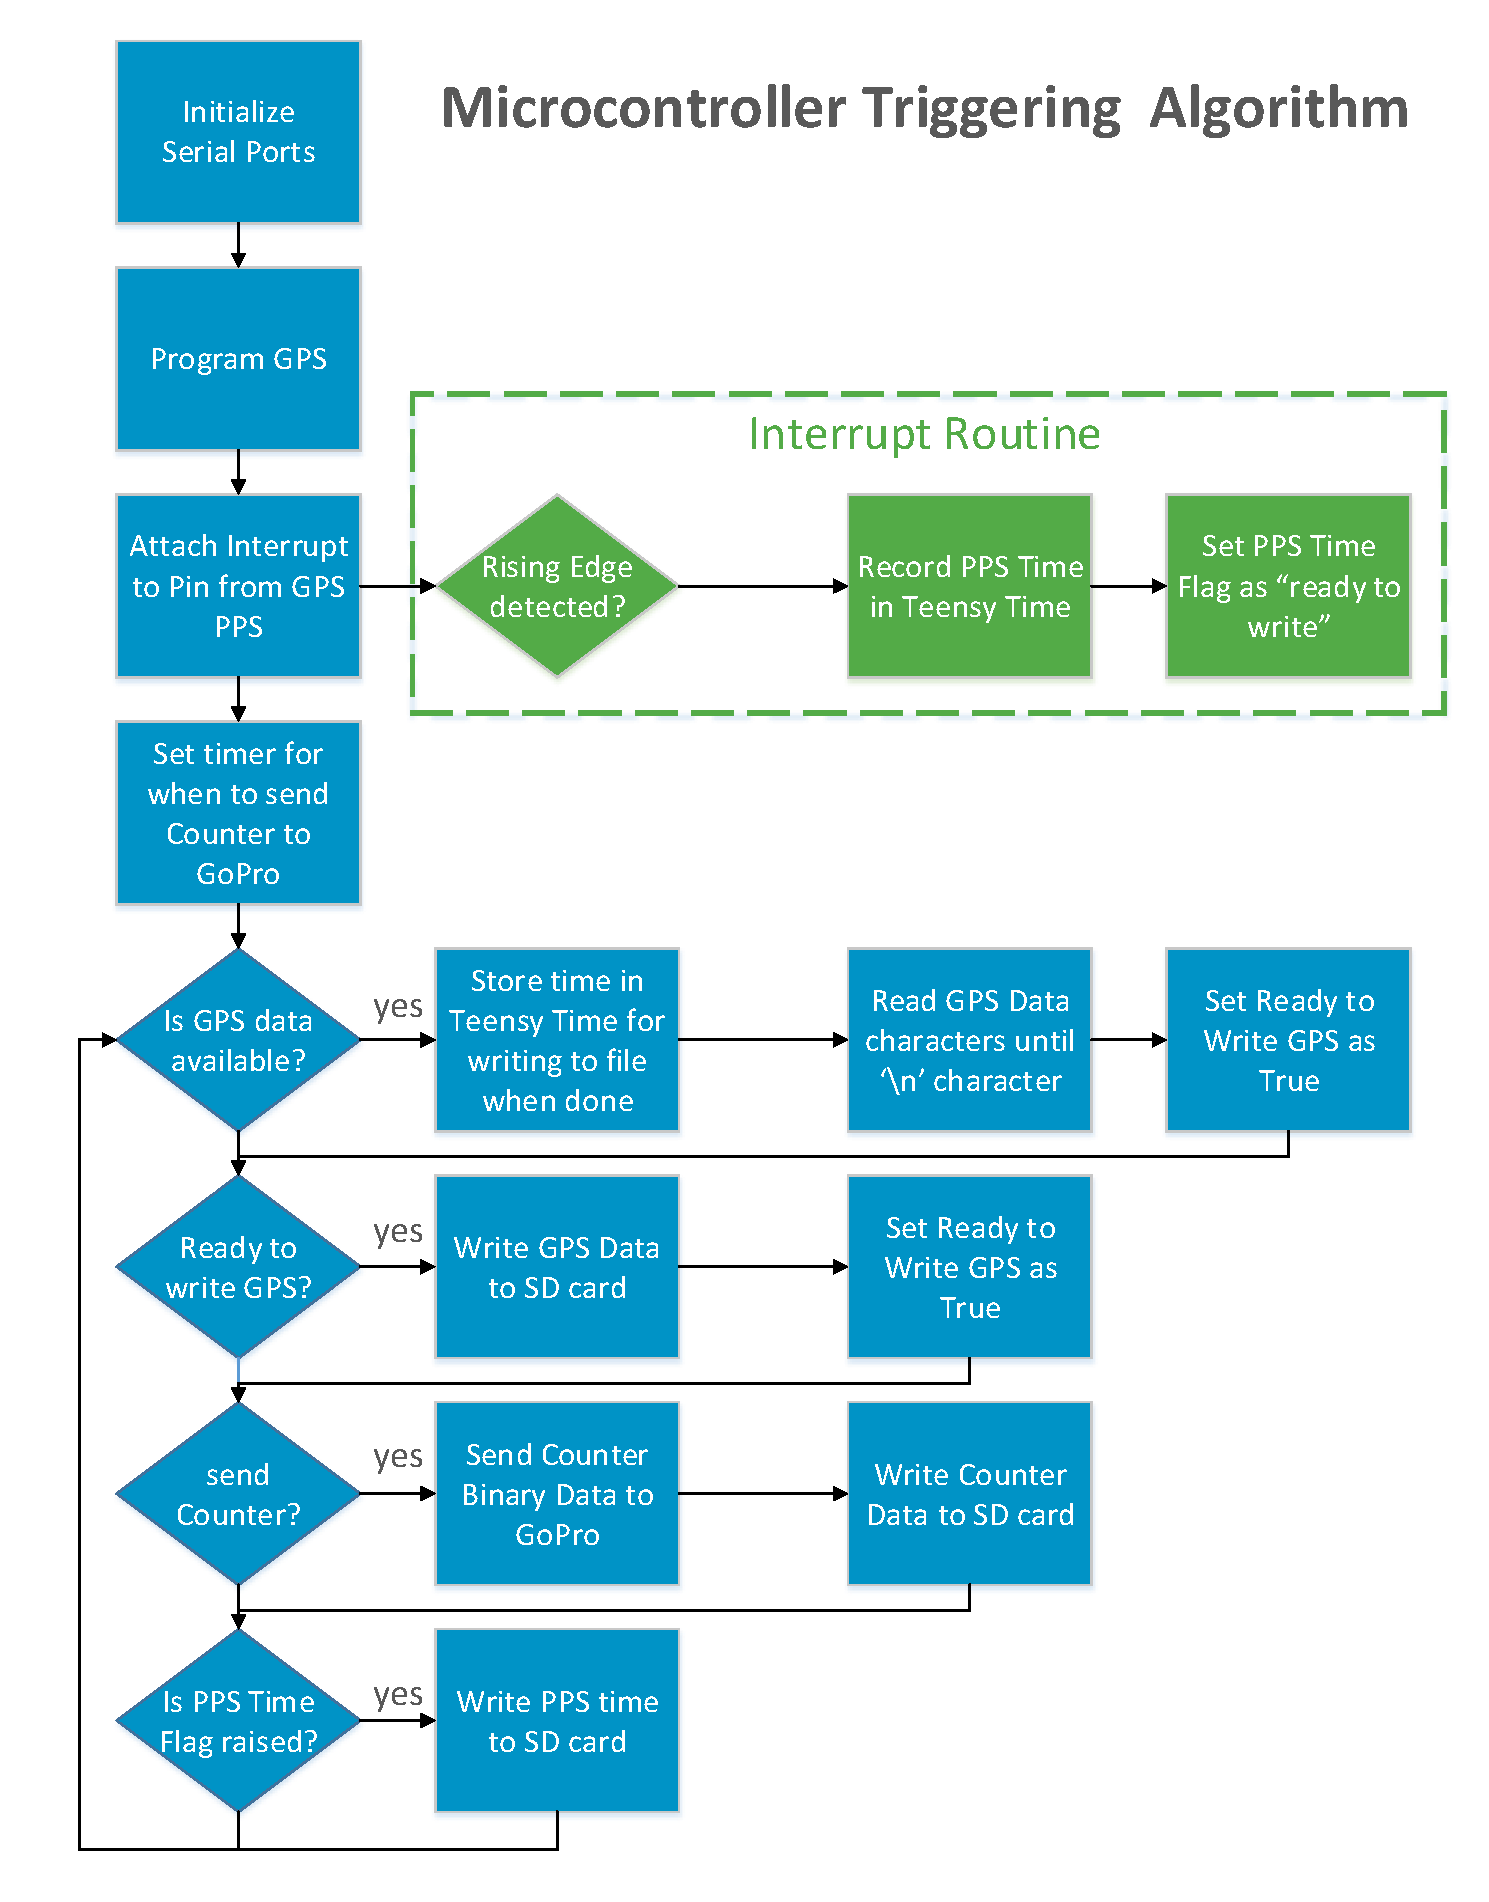
\includegraphics[scale = 0.4]{../figures/TeensyFlowchart.pdf}
	\caption{The Teensy algorithm is written to attempt to ensure as accurate timing synchronization as possible.  }
	\label{fig:TeensyFlow}
\end{figure}

The output log file is structured similarly to the NMEA format, but does not enact checksums for each line.  Each line of data is sent as a comma delimited line, where the first column is the address field, or identifier preceded by a `\$'.  The second column in each line is always the time in milliseconds from the time the microcontroller was turned on.  The relevant id fields are described in \tabref{tab:nmea}.  An example snippet of data from the file is shown in \figref{fig:nmea}.  A script for parsing the data is shown in \algref{alg:getValue}.
 \begin{table}[h]
 	\centering
 	\begin{tabular}{ll}
 		\toprule
 		ID & Description \\
 		\midrule
		\$MSG & Any Raw GPS NMEA Strings \\
		\$IND & Counter number that was sent to the GoPro \\
		\$PPS & No Info, besides the time it was received at \\
 		\bottomrule
 	\end{tabular}
 	\caption{The ID for each log file line is essential to parsing the data.}
 	\label{tab:nmea}
 \end{table}
 
 \begin{figure}[H]
 	\centering
 	\includegraphics[scale = 0.7]{../figures/logfileend.png}
 	\caption{The Teensy log file is recorded similarly to a NMEA structure, with each line beginning with an ID preceded by a `\$' symbol, and followed by the time in Teensy time.}
 	\label{fig:nmea}
 \end{figure}

\section{Potential Electronics Improvements}
\subsection{Fix Blunders in PCB Board}
There are a few improvements that could be made to the PCB and electronics for future versions.  The first improvement is an improved main PCB.  The PCB design used for this version had a few minor errors.  These error included: the DC-DC having to be mounted backwards, a slight offset of the IMU pins, and a few incorrect resistor values.  These fixes were manually implemented when the PCB was soldered together, and also electronically implemented in the board and schematic diagrams.  The new files are saved and have been delivered electronically.  
\subsection{Integrate onboard IMU}
The IMU is soldered to the board and connected to the SDA and SCL ports, however it is currently unrecorded.  The initial focus was to ensure accurate timestamping before adding in more read write cycles from the IMU.  While this IMU is very low cost, and low accuracy, it will most likely be able to provide a rough estimate of camera orientation.  
\subsection{Improve GPS Quality}
A large improvement would be to improve the quality of the GPS receiver.  The current L1 only GPS is accurate to less than 3m per the documentation, and does not record raw pseudo-ranges for post-processing.  Integration of a RTK GPS, L1 and L2 GPS, post-processing enabled GPS, or a fully integrated INS would greatly benefit the calculation of the camera pose and orientation.  The Ultimate GPS is placed into a socket on the PCB, with the thought that in the future an improved GPS sending NMEA strings could be integrated into the workflow with possibly only software modifications.
\subsection{Implement Charge Port and USB Hub}
A final improvement could be implemented to improve the usability of the system by adding a charge port and a USB hub to enable charging and reading from the sensors via one cable.  The current workflow for getting data out of the system involves removing the SD card or plugging a separate USB cable into the USB port.  An integrated switch on the Panel PCB could be a good place for a USB hub or a battery charging circuit.
	
	\chapter{Mount Design and Fabrication}		
	A mount was designed and fabricated to house the cameras and triggering electronics so that it could be mounted to a X8 UAV platform.  The constraints and goals of the design were as follows:
\begin{itemize}
	\item Weigh under 800g (X8 payload limit)
	\item House 4 GoPro cameras and triggering electronics
	\item Rigid, to ensure constant relative orientations between the cameras
	\item Easily manufactured for rapid prototyping and improvements
	\item Designed so cameras and electronics can be easily removed
	\item Little to no tools required
	\item Low cost 
\end{itemize}
\section{3D CAD Design}
Given the design constraints, it was clear that 3D printing using PLA or ABS plastic provided the most robust manufacturing methodology. The plastic is lightweight, easily manufactured, perfect for rapid prototyping, low cost, rigid, and can be designed with intricate interlocking parts to minimize the use of tools.  Each part of the sensor that was 3D printed was designed for 3D printing to minimize the amount of support required.  Each part has an optimal orientation that it should be printed at, so as to maximize structural integrity and minimize support. For example, a five sided hollow cube should be printed so that the open face is up, so that no support is necessary.  The orientation of each of the parts should be intuitive to the user.
	\subsection{Camera Enclosure Design}
	The GoPro camera enclosure, shown in \figref{fig:camEnclosure} was designed so that the cameras could be easily removed, as well as fit tightly into the enclosure so that there is no movement or shifting during the flight.  Many prototypes were generated, and various tolerances were investigated to ensure a compromise of ``easy to remove'' and ``doesn't move while in flight.''  A hinged design was selected as it minimized the number of screws or tools required, and was also a simple design to 3D print.  The lens protrudes into the threaded cylinder on the lid, and all of the ports and buttons are accessible.  The enclosure consists of 3 parts:
	\begin{enumerate}
		\item Enclosure (yellow): This is the main body that the GoPro mounts into
		\item Lid (red): This is the hinged part that locks the camera into place
		\item Cap (not shown): This 3D printed part threads onto the lid to protect the GoPro lens when the cameras is not acquiring imagery.
	\end{enumerate}
	The lid and cap are printed individually, while the enclosure is mounted to the Camera Mount in software, and printed as a fused, solid part, as shown in \figref{fig:mountcombo}.
	\begin{figure}[H]
		\centering
		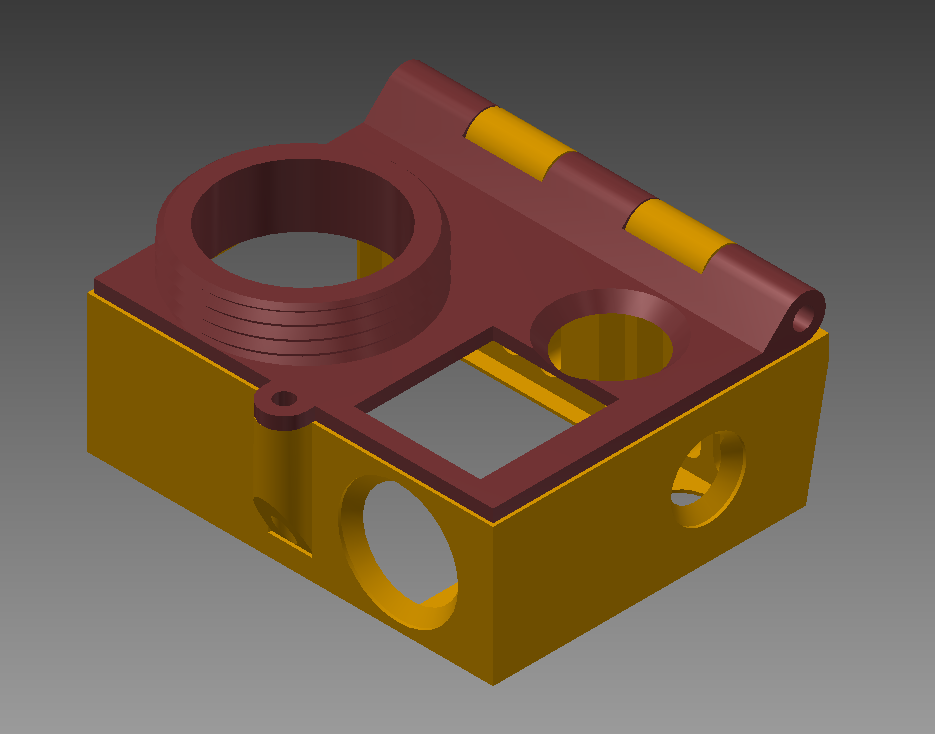
\includegraphics[scale = 0.4]{../figures/cad/cameraEnclosure.png}
		\caption{The camera enclosure was designed with a hinge, and one locking screw.  The threaded area around the cylinder for the lens enables a protective cap to be screwed on.}
		\label{fig:camEnclosure}
	\end{figure}

	\subsection{Camera Mount Design}
	The camera mount, shown in \figref{fig:mount}, defines the orientation of each of the cameras, and is the main frame of the design.  The camera enclosures are mounted directly to each of the four bottom planes in software, and together they are printed as one piece.  This print requires some support material to be removed, but ensures less tools and moving parts in the final design.  The proper orientation for printing the Camera Mount is with the wide opening for the electronics tray facing upwards, so that no support material is required within the body.

	The camera mount is designed so that the electronics tray can slide in and out such that the triggering electronics may be removed easily.  It also incorporates a honeycomb pattern on the top to reduce the overall weight of the system.  The four legs are designed so that vibration damping balls may be placed to connect the system to the X8 Quadcopter legs, shown in \figref{fig:legs}.  
	\begin{figure}[H]
		\centering
		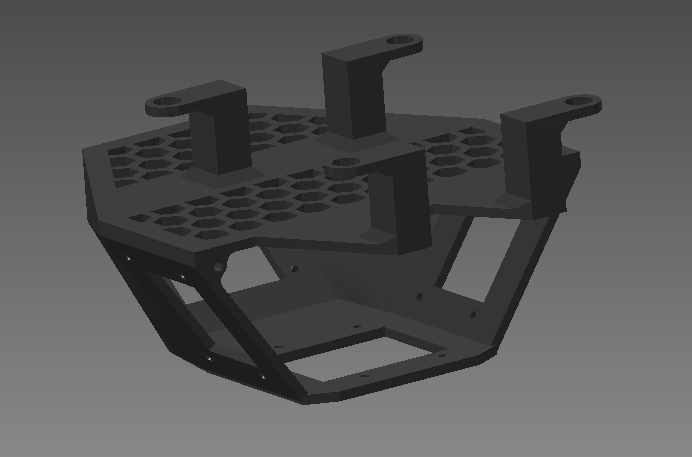
\includegraphics[scale = 0.4]{../figures/cad/mount.png}
		\caption{The camera mount was designed separately from the enclosure, so that the 4 cameras could be mounted to the design in software and they could be printed as one part.}
		\label{fig:mount}
	\end{figure}
	
	\subsection{Electronics Tray and Panel}
	The electronics tray, shown in \figref{fig:elec}, was designed for easy access to the electronics PCB, while still providing status lights and a power switch on the outside.  The tray is locked in with two screws in the upper corners, to ensure it does not slide out during a flight.  The panel portion of the tray, houses three status LEDs, a Voltage LCD display, a power switch, the panel PCB for connections, and an external antenna connection point.  The decoupling of the electronics tray from the mount allows for various electronics packages and batteries to be integrated into the system, without having to redesign a new mount.
	\begin{figure}[H]
		\centering
		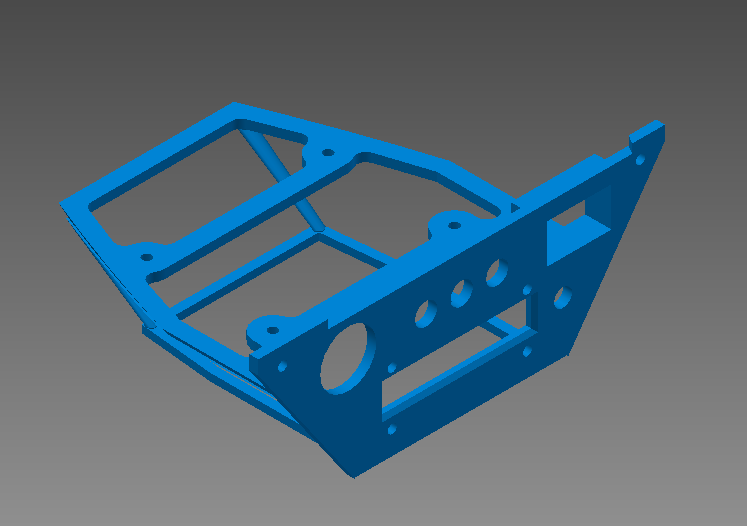
\includegraphics[scale = 0.4]{../figures/cad/electronicsTray.png}
		\caption{The electronics tray was designed so that the PCBs could easily be slid in and out, while the panel provided power and status lights.}
		\label{fig:elec}
	\end{figure}
		
	\subsection{X8 Quadcopter Legs Design}
	The X8 legs mount to the X8 chassis using three bolts.  These straddle the battery, and provide a socket for the vibration damping balls to be attached to.  These vibration damping balls, shown in \figref{fig:vibballs}, are integrated to reduce the propagation of vibration from the motors to the cameras.  Both 200g and 300g vibration damping balls were provided, as the optimum type has not been determined.  Based on the weight of the system, four 200g vibration damping balls should provide a good initial amount of vibration damping. 
	\begin{figure}[H]
		\centering
		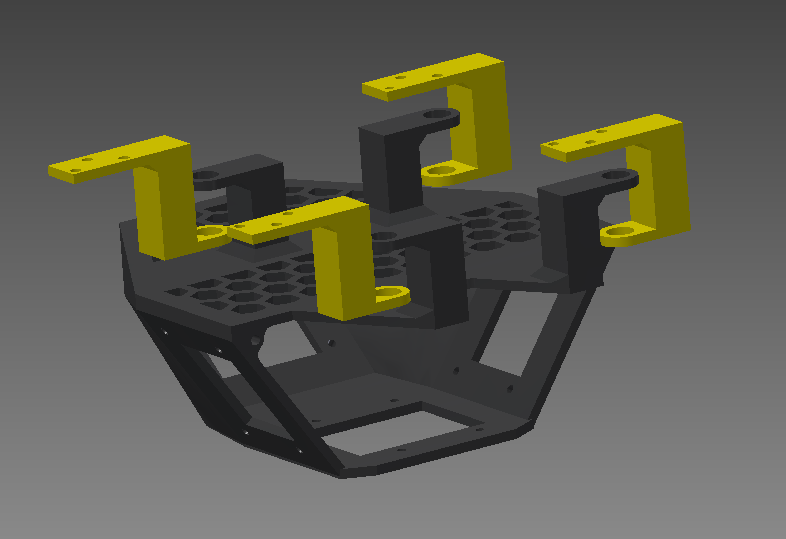
\includegraphics[scale = 0.4]{../figures/cad/bracket.png}
		\caption{The X8 legs were designed so that a vibration damping ball could be placed in between the legs to reduce vibration.}
		\label{fig:legs}
	\end{figure}

	\begin{figure}[H]
		\centering
		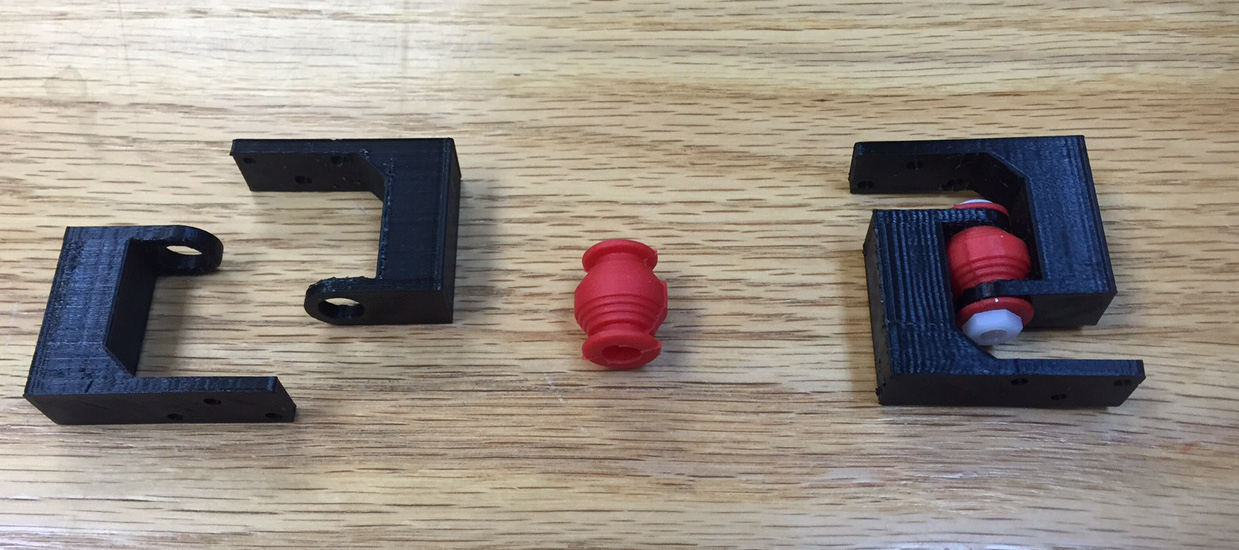
\includegraphics[scale = 0.25]{../figures/vibballs.JPG}
		\caption{The vibration damping balls, shown in red, are used to connect the X8 to the mount and reduce the vibration from the X8 motors.}
		\label{fig:vibballs}
	\end{figure}
	\section{Full Design Specs}
	The final system weighs ~700g with all of the cameras and electronics on board, and can be printed with one 1kg spool of printer filament.  The full system, shown in \figref{fig:mountcombo} is mounted to the X8 and can acquire imagery for approximately 15 minutes.  The fully mounted system is shown in \figref{fig:x8mounted}.  
	
	\begin{figure}[H]
		\centering
		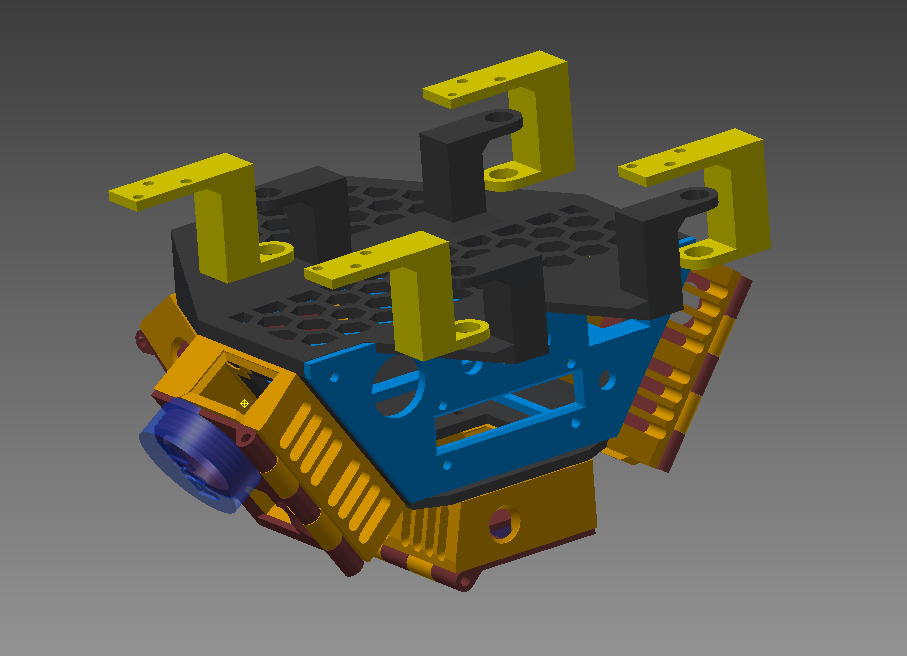
\includegraphics[scale = 0.4]{../figures/cad/all.png}
		\caption{The camera mount was designed separately from the enclosure, so that the 4 cameras could be mounted to the design in software and they could be printed as one part.}
		\label{fig:mountcombo}
	\end{figure}

	\begin{figure}[H]
		\centering
		\includegraphics[scale = 0.7]{../figures/mvssv2.jpg}
		\caption{The sensor is mounted to the bottom of the X8 with the GoPros installed for a proof of concept flight.}
		\label{fig:x8mounted}
	\end{figure}
	
	\section{Camera Orientations}
	One of the main benefits of the 3D printed CAD Design, is the relative orientations between the cameras can be measured in software.  Although there are sure to be uncertainties with printing and camera placement, the measured orientations should be very accurate.  In order to define the coordinate systems, a central `Mount coordinate system' is defined to align with the X8 body at approximately the center of the mount, as shown in \figref{fig:orient}.  The camera is defined such that the focal point of the camera is the origin, Z points outward from the camera, Y is down when the camera is facing upright, and X is along the length of the camera to the right.  The transformation from each camera to the mount is defined in a right handed coordinate system based on the Tait Bryant Euler angles.  The order of rotations is Z($\Psi$)-Y($\Theta$)-X($\Phi$), and the rotation is defined in \eqnref{eqn:rot}, where DCM represents the Direction Cosine Matrix.
	
	\begin{figure}[H]
		\centering
		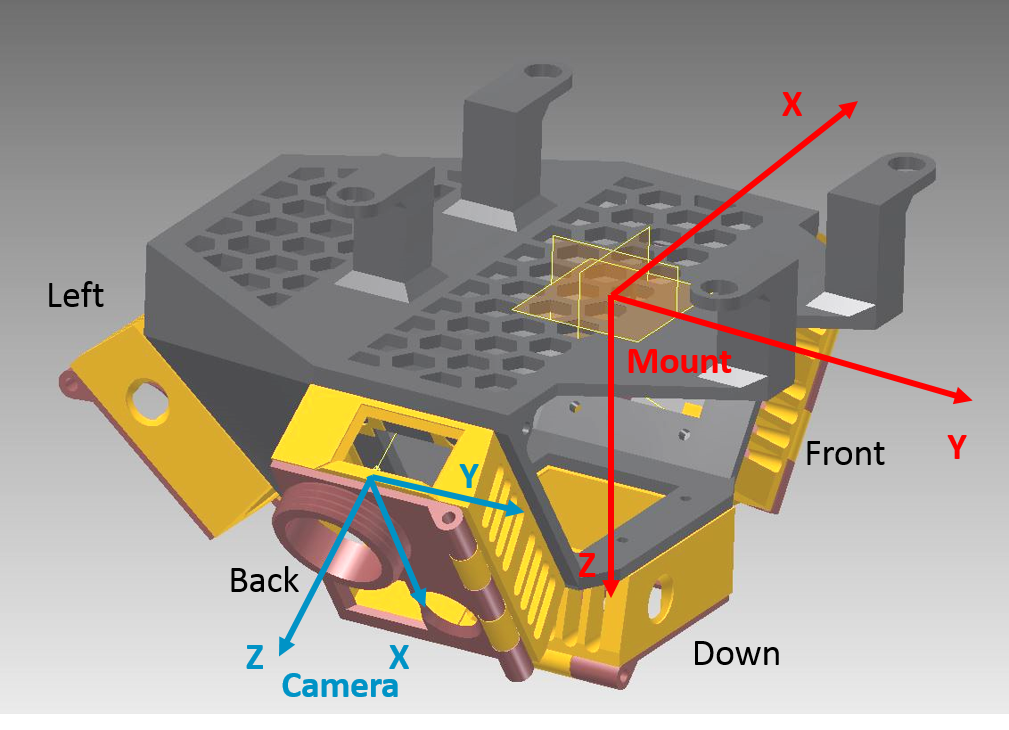
\includegraphics[scale = 0.4]{../figures/orient.png}
		\caption{The camera coordinate systems defined from the CAD model are relative to the mount coordinate system, which is defined as an arbitrary point on the top center of the mount.}
		\label{fig:orient}
	\end{figure}
	
% Table generated by Excel2LaTeX from sheet 'Sheet2'
\begin{table}[htbp]
	\centering
	\caption{The rotation and translation from the camera coordinates to the mount coordinates is defined in a right hand coordinate system where Yaw, Pitch, and Roll are defined as right hand rotations about the Z,Y, and X axes respectively.}
	\begin{tabular}{lcrrrrrr}
		\toprule
		Camera Name & Lens (mm) & Yaw($\Psi $) & Pitch($\Theta$) & Roll($\Phi$) & X (in) & Y (in) & Z (in) \\
		\midrule
		\multicolumn{1}{l}{Back} & 2.9   & 0\degree     & 55\degree    & 0\degree     & 2.74 & 0.904 & -0.931 \\
		\multicolumn{1}{l}{Down} & 5.4   & -90\degree   & 0\degree     & 0\degree     & -0.404 & 1.014 & -2.587 \\
		\multicolumn{1}{l}{Front} & 2.9   & 0\degree     & -55\degree   & 0\degree     & -2.085 & 0.904 & -1.867 \\
		\multicolumn{1}{l}{Left} & 2.9   & 180\degree   & 0\degree     & 40\degree    & -0.571 & 3.558 & -1.92 \\
		\bottomrule
	\end{tabular}%
	\label{tab:imRotations}%
\end{table}%
\begin{align}
\label{eqn:rot}
X_{mount} = R\times X_{camera} + T \\ 
\nonumber
R = DCM(\Psi,\Theta,\Phi)
\quad
T = \begin{bmatrix}
X \\ Y \\ Z
\end{bmatrix}
\end{align}

	\section{Possible Improvements}
	\subsection{Reduce Weight}
	The current sensor design weights about 700g, but not much optimization in the design for weight reduction has been performed.  If there is a large potential benefit that could be gained from a reduction in weight, the current mount and designs have some room to remove material while maintaining rigidity.  An alternative method, while more intensive, would be to incorporate carbon fiber or some other material onto the 3D printed parts to increase rigidity.  
	\subsection{Implement Weatherproofing}
	Sand or moisture can currently get into the electronics enclosure through the honeycomb pattern on the top of the mount.  If this becomes a noticeable issue, the mount should be redesigned to seal off this opening. This could be achieved with something as simple as tape across the gaps, or by adding a thin layer in the CAD design.  If the sensor is to be used in harsher environments, it could be redesigned with gaskets and more robust sealing mechanism to become more fully weatherproof.
	\subsection{Improve Panel}
	The first version of the panel contains various lights and LEDs to keep the user knowledgeable on the status of the sensor.  This panel could be modified to either add or remove status leds, or even a small LCD screen for text status updates.  If the status lights and LCDs are determined to not be useful, `improvement' could actually mean removing some components.
	\subsection{Improve Vibration Damping}
	The vibration damping implemented is a first cut, low cost approach to attempt to remove the vibration from the system.  If this method is not adequate, further investigation into vibration damping systems will need to be performed.  The design of the mount is modular enough that the only changes would be to the Legs of both the X8 bracket and the mount.  
	
	\chapter{Image Synchronization}\label{ch:sync}
		The cameras are each synchronized to UTC time using the audio data and PCB log file.  Once each camera is synchronized to UTC time, frames are extracted at regular intervals for each video, and these images are said to be ``synchronized.''  These videos are not however, hardware triggered and therefore the shutters are not synchronized.  The theoretical accuracy of this methodology results in the cameras synchronized to a worst case scenario of 1/30s when ignoring all other sources of noise.
	
	\section{Technical Approach}
	The algorithm to develop the synchronization of the cameras from GoPro time to UTC time was developped in Matlab.  The logfile, as described in Section \ref{sec:algoLog}, records the GPS data, PPS rising edge time, and the time the binary count value was sent to the GoPro.  The GoPro audio channels recorded the PPS signal and the binary count value from the Teensy microcontroller.  Each of these data has redundant observations between the time frames, which enable us to perform a least squares adjustment between each of the time frames.  When the processing is complete, p1 and p2 coefficient values as described in \eqnref{eqn:utc2gopro}, are recorded in a text file.
	
	\begin{equation}
	\label{eqn:utc2gopro}
	t_{UTC} = p1 \times t_{gopro} + p2 
	\end{equation}
	
	The processing is broken up into four main algorithms:
	\begin{enumerate}
		\item Calculate GoPro time to UTC time coefficients
		\item Extract Frames from GoPro Video at UTC times 
		\item Convert logfile into a CSV file with GPS info and UTC timestamps
		\item Interpolate GPS position info for each image based on corresponding UTC times 
	\end{enumerate}

	\subsection{GoPro to UTC time}
	
	\subsubsection{GoPro Audio Signal Decoding}

	One challenge with extracting the binary and PPS data from the audio channel of the GoPro was filtering out the GoPro signal conditioning of the input signal.  For example, \figref{fig:rawPPS} demonstrates how a square PPS signal appears in the recorded audio file.  Notice how the PPS signal, which should be a square wave, actually decays to 0 despite the voltage.  Therefore, an algorithm was written to detect large changes in signal, which then represent changes in voltage.  For the PPS signal, the detection of rising and falling edges of the PPS pulse was trivial, but it became slightly more complicated for the binary signal.
	\begin{figure}[H]
		\centering
		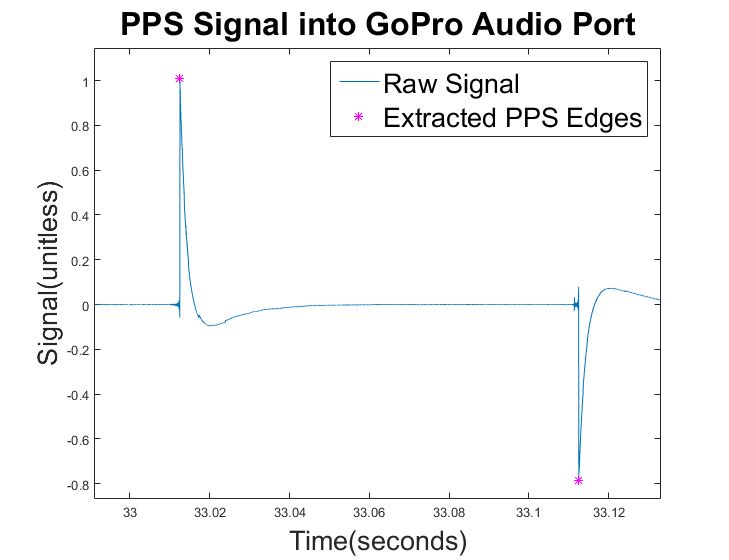
\includegraphics[scale = 0.7]{../figures/rawPPS.png}
		\caption{The PPS, which should be represented as a square wave, actually decays to 0 regardless of the voltage. The algorithm therefore is written to detect the large gradients, which represent a change in voltage.}
		\label{fig:rawPPS}
	\end{figure}
	The binary signal is set to 300 baud in the Teensy algorithm however it actually is sent at 1660 baud.  This is acceptable, as the peaks were still discernable at this baud rate.  If however, a faster baud rate were used, the peaks would become too close together and be difficult to decode.  \figref{fig:rawNMEA} is an example decoded binary signal.  The data is sent at 8N1 with no parity, so for the 2 byte binary integer being sent, it uses 20 bits.  The raw signal is filtered to detect large changes, then a Gaussian filter is applied to smooth out the data.  The peaks are then extracted at the known baud rate, with a peak threshold set as 1/3 the absolute value of the max peak value.  The signal is then decoded into a binary signal, using an algorithm that takes into account that the signal will only change when the bit is changing.  For example, notice how the 17th bit is high, and the 18th bit is 0, but both those values represent a 1 in binary.  The bit value does not change to 0 until a low peak is detected at bit 19.  
	
	\begin{figure}[H]
		\centering
		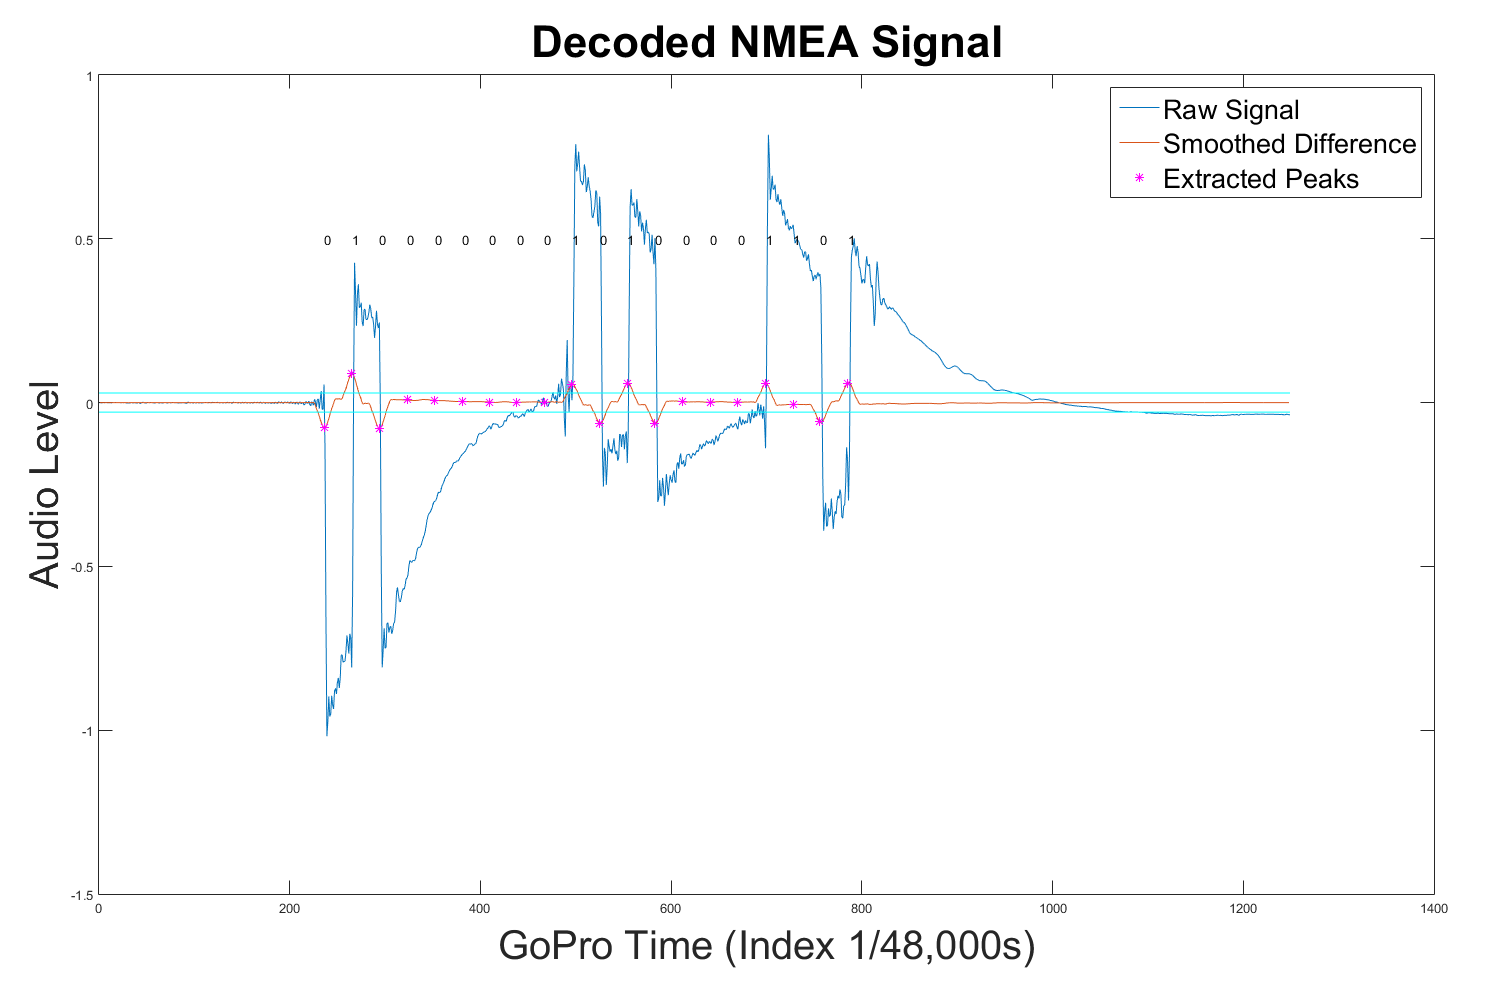
\includegraphics[scale = 0.4]{../figures/decodedNMEA.png}
		\caption{The binary signal sent to the audio port suffers the same decay as shown in the PPS signal.  Here, the change in signal was used to detect when a change in bit value occurred.}
		\label{fig:rawNMEA}
	\end{figure}
	
	\subsubsection{Algorithm Pseudocode}
		The conversion from GoPro time to UTC time can be performed without a PPS signal, but the absolute quality of this conversion will suffer due to latency in the Serial NMEA port and buffering.  However, the relative synchronization between the cameras should remain the same, as any latency in reading the Serial port will be constant across each camera.  The different time frames and data exchange between the Teensy, GoPro, and GPS PPS are shown in \tabref{tab:timeframes}.  Note that there is an ambiguity when attempting to correlate two PPS signals, as the PPS signal simply refers to a start of a second.  If two PPS triggers are detected in two different time frames, there is no direct way to correlate the two.  For this reason, GPS data sends NMEA strings to put the PPS second into an absolute UTC time frame.  The function to calculate this offset and save a text file has been electronically delivered, and is also shown in \ref{sec:calcGopro2GPStime}.  
	
		\begin{table}[htbp]
			\centering
			\caption{The different data exchanges are recorded in three different time frames.  Note that the X represents a direct correspondence between the data, while a `*' represents an ambiguity in the correspondence. The PPS values are sent at the beginning of each second in time, but there is no context to what actual second it is.}
			\begin{tabular}{| l | c | c | c |}
				\hline
				Time Frame & Index & GPS NMEA & GPS PPS \\
				\hline
				GoPro & X     &       & * \\ 			\hline
				Teensy & X     & X     & X \\ 			\hline 
				UTC   &       & X     & * \\
				\hline
			\end{tabular}%
			\label{tab:timeframes}%
		\end{table}%
		
		The steps to achieve time synchronization between GoPro time and UTC time are outlined below:
		\begin{enumerate}
		\item Extract All data from the SD card and the GoPro Audio
		\item Use correspondences between Teensy Time and GoPro time for the index counter sent to the audio channel to calculate the conversion between the two time frames.
		\item Use the NMEA GPS string recorded in Teensy time and stamped with UTC time to calculate a conversion between Teensy time and UTC time.  *NOTE, if no PPS is detected, the algorithm stops here
		\item A PPS pulse is described as having a rising edge exactly on the second with precision to the nanosecond.  Using this knowledge, and the PPS timestamps in Teensy Time, estimate each PPS time in UTC time.  Round the value to the nearest second after using the Teensy to UTC conversion
		\item Convert the GoPro PPS times to UTC time, and round to the nearest PPS in UTC time.  This assumes that the time is accurate to less than 0.5 seconds, so that the rounding does not become out of phase.
		\item Calculate a new conversion from GoPro time to UTC time using the PPS correspondences.
		\item Save this information to a text file `*\_gopro2gps.txt.'
		\end{enumerate}
	
	\subsection{Extract Frames}
	Frames are extracted from the video imagery using the known conversion from GoPro time to UTC time, and a user-defined vector containing the times to extract imagery at.  The algorithm to extract these frames and save imagery and metadata is provided electronically and also located in \ref{sec:extractFrames}. The pseudocode for the algorithm to extract frames is as follows:
	\begin{enumerate}
		\item Read the MP4 Video file into Matlab using Matlab's \textit{VideoReader} Class
		\item Read the previously calculated goPro to UTC time constants
		\item Using the user input vector of desired UTC times for frames, calculate the correct frame indices to extract imagery
		\item Write each frame to a JPG in a user defined folder, and save an `iminfo.txt' CSV file which contains 3 Columns.  In order to quantify the timing errors, the actual and desired times are both written.  An example output file is shown in \figref{fig:iminfo}
		\begin{itemize}
			\item Image Name
			\item Image Actual Time (This is the actual time of the frame)
			\item Image Desired Time (This is the time the user wanted the frame at)
		\end{itemize}
	\end{enumerate} 
	
	\begin{figure}[H]
		\centering
		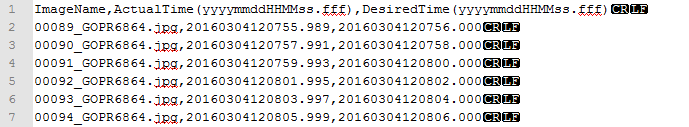
\includegraphics[scale = 0.8]{../figures/iminfotxt.png}
		\caption{The image info text file is comma delimited and is used to store metadata about the extract video frames.}
		\label{fig:iminfo}
	\end{figure}
	
	One issue that arose is that Windows machines running operating systems that predate Windows 10 do not contain the codecs for reading 4K video by default.  Since Matlab relies on these codecs, the Matlab \textit{VideoReader} class throws an error when attempting to read a 4K video file.  This issue is alleviated by instaling 3rd party codecs.
	
	A second issue that may arise is the use of the \textit{read} function is flagged bt Matlab as subject to removal in future versions of Matlab.  This function is used, rather than the new \textit{readFrame} function, as the \textit{read} function enables a frame to be read based on an index value.  The \textit{readFrame} function requires you to read each frame sequentially, which takes a lot of unnecessary time when you are reading every N frames.  
	\subsection{Convert Log file to CSV}
	\label{ssec:convertLog2CSV}
	The log file that is recorded on the SD card contains L1 GPS data which can be used to provide an initialization for the camera position when running Structure from Motion algorithms.  A quick algorithm to decode the log file and convert it from NMEA to a more easily interpretted CSV is provided electronically.  An example resultant file is shown in \figref{fig:gpstxt}.  This file is simply raw time and GPS position data, but it can be leveraged to interpolate camera positions, as described in \ref{ssec:InterpGPS}.
	
	\begin{figure}[H]
		\centering
		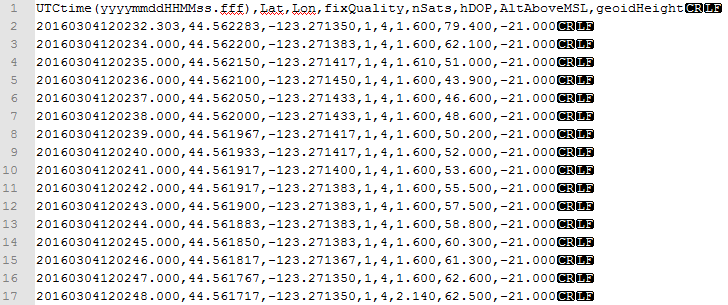
\includegraphics[scale = 0.6]{../figures/gpstxt.png}
		\caption{The log file is turned into a CSV file so that the GPS data can be easily extracted and leveraged.}
		\label{fig:gpstxt}
	\end{figure}
	
	\subsection{Interpolate GPS data for each image}
	\label{ssec:InterpGPS}
	Once all of the imagery has been extracted, estimated camera pose positions can be calculated using various sources of GPS data.  \figref{fig:postxt} demonstrates an example metadata file generated from the logfile gps positions.  The algorithm, shown in \ref{sec:addPositionInfo}, is developped to be modular so that any CSV file can be used to add position or other temporal metadata to the imagery.  The CSV file must have:
	\begin{enumerate}[a)]
		\item headers to describe the data, as these are propagated through to the merged metadata file
		\item A first column representing UTC time in the format `yyyymmddHHMMss.fff.'
	\end{enumerate}
	If these parameters are met, other sensor data such as that from the autopilot can be easily integrated into the workflow.
	
	\begin{figure}[H]
		\centering
		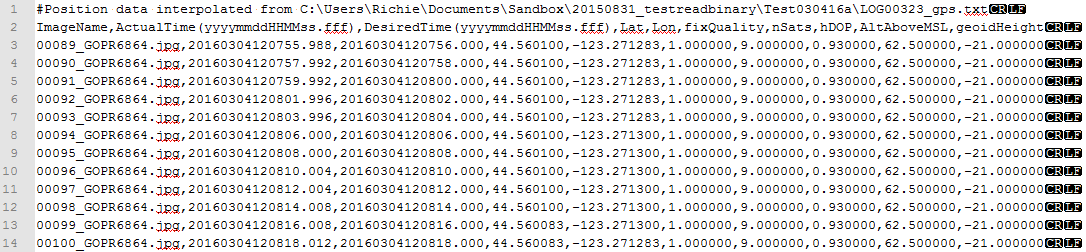
\includegraphics[scale = 0.6]{../figures/postxt.png}
		\caption{The GPS data is appended to the image position metadata so that each image has interpolated GPS values.}
		\label{fig:postxt}
	\end{figure}
	
	\section{Temporal Accuracy}
	The temporal accuracy was tested by observing a cell phone that was updating with the UTC time via a website.  This test is limited greatly by a number of factors, included refresh rate of the phone screen, refresh rate of the website, and the displayed temporal resolution of the website is only to the second.  Initial results show that the time is correctly synchronized to UTC time, in the sense that the times appear to match relatively well with what is shown on the screen, as shown in \figref{fig:badsync}.
	
	\begin{figure}[H]
		\centering
		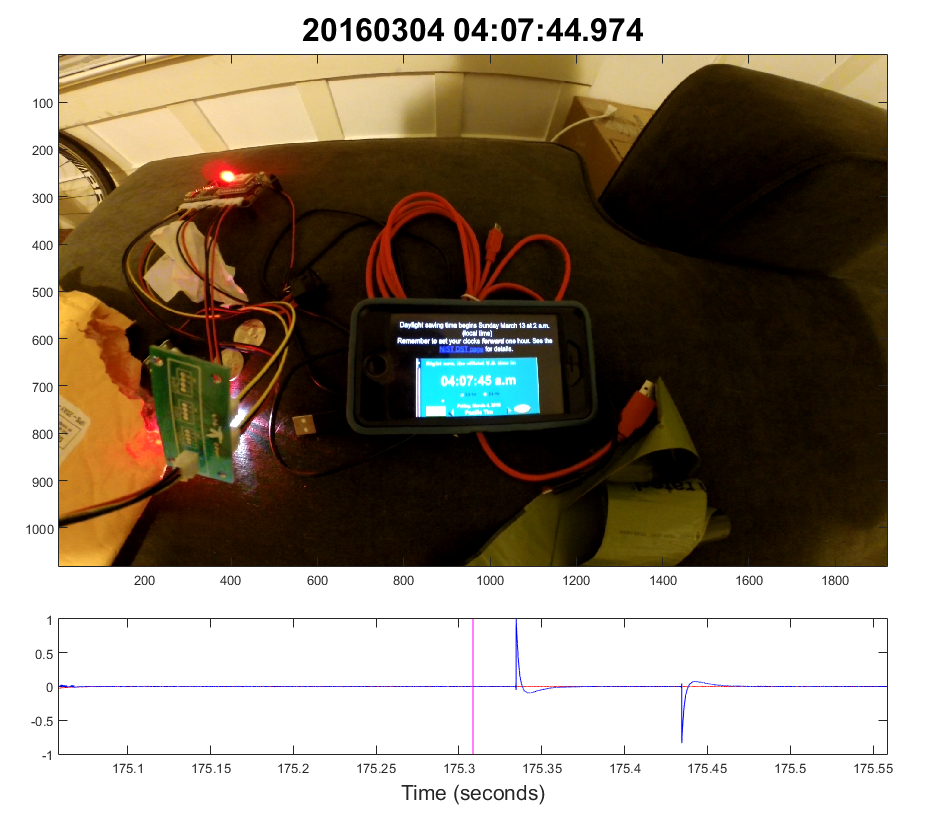
\includegraphics[scale = 0.6]{../figures/badsync.png}
		\caption{The synchronization of the imagery was tested using a cell phone updating via a time server to UTC time.  The top pannel shows the imagery, and the bottom panel shows the PPS signal channel of the audio.  The magenta line represents the current time. Notice that the white, PPS light under the green PCB is on, before the signal is shown in the audio.}
		\label{fig:badsync}
	\end{figure}
	
	However, one issue that was observed is the latency between the video and the audio channel within the GoPro.  GoPro cameras are consumer grade cameras, and therefore time synchronization between the audio and video does not need to be perfectly precise.  Notice in \figref{fig:badsync} how the white PPS light under the PCB is lit up before it is recorded on the audio channel.  This indicates that the Video signal is farther ahead in time than the audio channel.  This offset was observed to be consistently one to two frames off, but further tests would need to be done to make any statements about it's consistency.  Hopefully, the latency between the audio and video port is a constant offset that can be calculated once and applied to each camera.  Further tests will need to be done to fully quantify the accuracy of this methodology due to other sources of error.	
	
	\section{Possible Improvements}
	\subsection{Embed x8 Flight log info}
	The X8 Pixhawk autopilot records position and orientation values directly to the SD card in the Pixhawk.  These data can be read into the 3D Robotics ``Mission Planner'' software, and converted into a Matlab file.  Once the data is in Matlab, it should be saved as a CSV, as described in \ref{ssec:convertLog2CSV}.  While the autopilot is not rigidly mounted to the cameras, it should provide a more accurate camera pose estimation than what could be derived from the onboard 9dof IMU.
	\subsection{Incorporate onboard IMU}
	If however, the vibration damping between the camera and the X8 autopilot significantly invalidates the ``rigid body'' assumption, the onboard IMU could be used to generate improved position and orientation values.  A Kalman filter should be implemented to generate an improved trajectory than what could be generated from just the raw data.  One issue that will need to be overcome in order to integrate this system, is to modify the Teensy code to record the raw 9dof measurements.  These raw values have been excluded from this iteration, as there was concern that reading and writing from another sensor could cause latency and delays in the time synchronization section of the code.  Further tests will be required to ensure that this is not the case.
	
	\chapter{Acquisition and Data Storage}
		\section{Mission Planning Tool}
	To aid in development of a mission plan, a flight planning tool was developed to assess dwell time at various altitude and speeds.  The tool, \textit{mvss\_cameraFlightPlanning2}, allows the user to manually input flight parameter constants of altitude, flight speed, and image frame rate, as shown in \algref{alg:flightplan}.  
	
	\lstinputlisting[
	caption = {The flight planning tool is used to assist with calculating dwell time and spatial coverage for various flight parameters.},
	label = {alg:flightplan},
	style = Matlab-editor,
	basicstyle = \mlttfamily,
	firstline = 1,
	lastline = 7
	]{../../Matlab/mvss_cameraFlightPlanning2.m}
	
	The \textit{mvss\_cameraFlightPlanning2} algorithm automatically generates two plots, shown in \figref{fig:flightplots}.  The left plot is a spatial snapshot, showing what one image from each of the four cameras will cover spatially when it is centered at (0,0).  In the example shown, the images cover the entire 4km grid in the along-track distance.  The right plot shows the time dwell that each location would be imaged assuming a constant flight speed and altitude.  Higher, red values, represent a longer dwell time.  Each camera configuration yields a slightly different heat map of values, which can be useful for planning flight speeds and planning coverage.
		
	\begin{figure}[H]
		\centering
		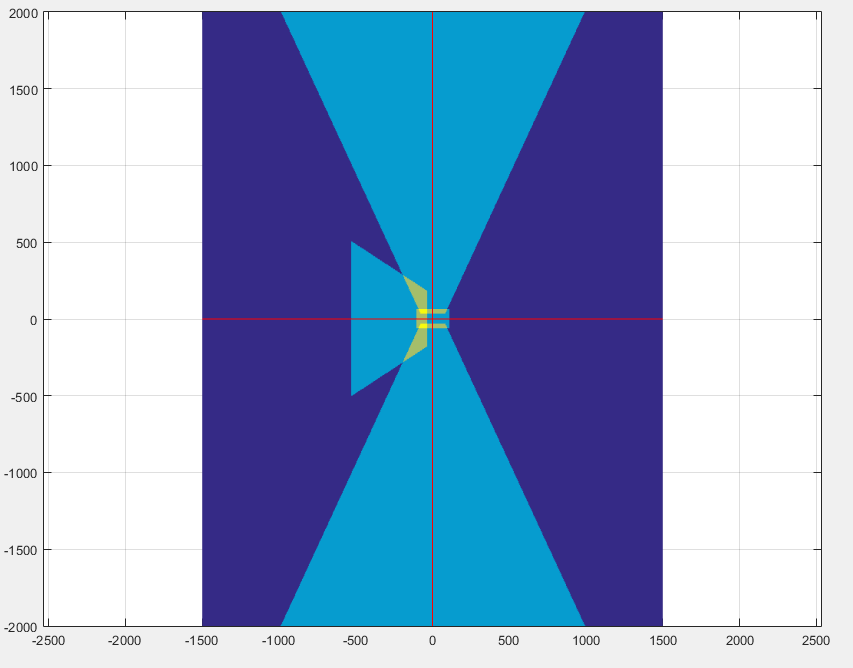
\includegraphics[scale = 0.3]{../figures/imageoverlap.png}
		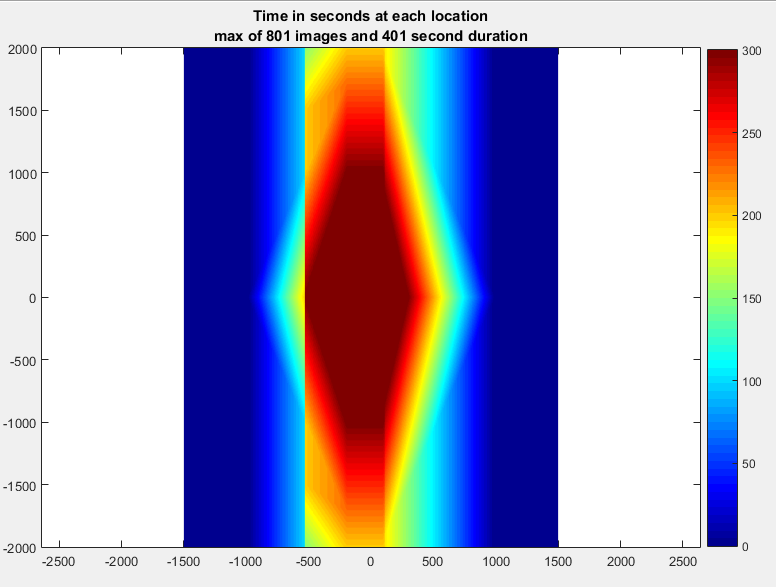
\includegraphics[scale = 0.341]{../figures/dwell.PNG}
		\caption{(Left) The spatial extent of one image snapshot is plotted with cross-track distance on the X-axis, and along-track distance on the Y-axis. (Right) The dwell time at every location in the cross-track(x-axis) and along-track(y-axis) is colored based on time in seconds, assuming a constant flight speed and altitude.}
		\label{fig:flightplots}
	\end{figure}
	\section{Flight Checklists}
	Three initial checklists are provided to ensure accurate and reliable data acquisitions.  The first checklist represents what should be done prior to a flight.  This includes checking all connections, batteries, SD cards, and settings to find any bugs before the actual acquisition.  The second checklist is to be used during the actual data collect.  This list should be improved to include more detailed X8 flight checklists, provided by 3DR robotics.  The final checklist describes how data should be stored and organized after a data collect.  This organization of data will make processing much more intuitive and user friendly. These checklists should be seen as an initial start, and should be iterated upon and improved based on user experience.
	\cleardoublepage
	\subsection{Pre Flight Checklist}
	\subsubsection*{Day Before Flight}
	\begin{easylist}[checklist]
		&& Charge GoPro Batteries
		&& Check Voltage/Charge PCB Batteries
		&& Clear SD Card for each camera
		&& Insert SD card for each camera
		&& Test Electronics to ensure it turns on and acquires PPS
		&& Clear SD card for electronics (DO NOT CLEAR CONFIG FILE)
		&& Make sure the config file still says 115200 Baud
		&& Place SD card for electronics into PCB slot
		&& Install Sensor on X8
		&& Charge Battery for X8
		&& Upload Mission to X8		
	\end{easylist}
	\subsubsection*{Once batteries are charged}
	\begin{easylist}[checklist]
			&& Install electronics tray
			&& Turn on electronics and ensure power light comes on and voltage is good
			&& Turn off electronics so power light goes off
			&& Ensure cameras turn on and are functional
			&& Ensure camera settings are set to 4K mode
			&& Place cameras in enclosures
			&&& Make sure each camera is in it's corresponding spot based on focal length
			&& Lock down each camera with screw
			&& Ensure cameras turn on and are functional after locking down
			&& Turn cameras all off so not to drain battery
			&& Place Cap on cameras to protect lenses
			&& Plug in the trigger cables, and handle cable management
			&& Plug in external GPS, and handle cable management
			&& lock down electronics tray with screw
	\end{easylist}
	
	\subsubsection*{One Hour before Flight}
	\begin{easylist}[checklist]
		&& Check Electronics	
		&&& Turn on electronics and ensure power light comes on and voltage is good
		&&& Turn off electronics so power light goes off
		&& Check Cameras
		&&& Ensure cameras turn on and are functional
		&&& Ensure camera settings are set to 4K mode
		&&& Ensure SD cards are in cameras
		&&& Power off all cameras
		&& Check X8
		&&& Check X8 Battery Voltage
	\end{easylist}
	\cleardoublepage
	\subsection{Flight Checklist}
	\begin{easylist}[checklist]
		&& Place X8 with sensor where you want to take off from
		&& Unscrew lens caps
		&& Power on Electronics. Do not power off until done with collect.
		&& Wait until White Light is Flashing, signifying PPS (may take a minute)
		&& Power on X8 and initialize
		&& Wait until X8 is initialized and ready to takeoff
		&& Turn on Each camera
		&& Ensure each is set to 4k mode
		&& Press record on each camera
		&& Set X8 flying
		&& Land X8
		&& Stop recording on each camera
		&&& Make note of any cameras are off
		&&& Make note of the PPS status 
		&& Turn off the Electronics via the panel switch
		&& Turn Off X8
		&& Place Lens Caps on sensor to protect lenses
	\end{easylist}
	
	\cleardoublepage
	\section{Post Flight Checklist}
	\begin{easylist}[checklist]
		&& Extract Data and organize, per \ref{sec:rawdata}
		&&& Different `data collect ID' should be saved for each collect on a day
		&&& Extract the logfileNNN.txt from PCB SD card
		&&& Extract Each Camera *.MP4 files
		&&& Extract SD card, from the X8FlightLog from the autopilot 
		&& Task someone with processing the Lidar or GPS surveys
		&& Charge GoPro Batteries
		&& Charge PCB battery
		&& Double check all data is backed up
		&& Triple check all data is backed up
		&& Clear SD cards
		&&& Clear Camera SD cards
		&&& Clear Log SD card (except config file)
		&&& Clear X8 SD card
		&& Place SD cards back in cameras, PCB, and X8
		&& Store equipment
	\end{easylist}
	\cleardoublepage
	\section{Data Management}
	\subsection{Raw Data Structure}\label{sec:rawdata}
	\dirtree{%
		.1 \treeDB{DataDepot}.
		.2 \treeFolder{MVSS2}.
		.3 \treeFolder{yyyymmdd\_$<$datacollectID$>$}.
		.4 \treeFolder{data}.
		.5 \treeFolder{control}.
		.6 \treeTxt{gcps.txt}.
		.6 \treeLAS{LidarControl.las}.
		.5 \treeFolder{video}.
		.6 \treeFolder{$<$ Camera Name $>$ (eg. Back, Down, Front, Left)}.
		.7 \treeGopro{*.mp4}.
		.5 \treeFolder{log}.
		.6 \treeTxt{yyyymmdd\_$<$id$>$\_X8flightLog.txt (log from autopilot)}.
		.6 \treeTxt{yyyymmdd\_$<$id$>$\_LogNNNN.txt (log from electronics sd card)}.
		.5 \treeTxt{meta.txt (metadata text file created for each flight)}.
	}
	\cleardoublepage
	\subsection{Processed Data Structure}
	\dirtree{%
		.1 \treeDB{DataDepot}.
		.2 \treeFolder{MVSS2}.
		.3 \treeFolder{yyyymmdd\_$<$datacollectID$>$}.
		.4 \treeFolder{data}.
		.5 \treeFolder{control}.
		.6 \treeTxt{gcps.txt}.
		.6 \treeLAS{LidarControl.las}.
		.5 \treeFolder{video}.
		.6 \treeFolder{$<$ Camera Name $>$ (eg. Back, Down, Front, Left)}.
		.7 \treeGopro{*.mp4}.
		.7 \treeTxt{$<$mp4name$>$\_gopro2gps.txt}.
		.5 \treeFolder{imagery}.
		.6 \treeFolder{$<$ Process Name $>$ (eg. dt0pt5s, dt2s)}.
		.7 \treeFolder{$<$ Camera Name $>$ (eg. Back, Down, Front, Left)}.
		.8 \treeImg{\%06.0f\_$<$mp4name$>$.jpg}.
		.8 \treeTxt{iminfo\_$<$mp4name$>$.txt}.
		.8 \treeTxt{iminfo\_$<$mp4name$>$\_pos.txt}.
		.5 \treeFolder{log}.
		.6 \treeTxt{yyyymmdd\_$<$id$>$\_X8flightLog.txt (log from autopilot)}.
		.6 \treeTxt{yyyymmdd\_$<$id$>$\_LogNNNN.txt (log from electronics sd card)}.
		.6 \treeTxt{yyyymmdd\_$<$id$>$\_LogNNNN\_gps.txt (log from electronics sd card)}.
		.5 \treeTxt{meta.txt (metadata text file created for each flight)}.
		.4 \treeFolder{products}.
		.5 \treeFolder{pointcloud}.
		.6 \treePhotoscanFolder{$<$PhotoScan Project Name $>$}.
		.6 \treeTxt{photoscanlog.txt (point photoscan to save all commands to a logfile here)}.
		.6 \treeFolder{LAS}.
		.7 \treeLAS{$<$Pointcloud Name$>$.las (eg. Dense10GCPS, Optimzed5GCPs)}.
		.7 \treeTxt{$<$Pointcloud Name$>$\_meta.txt}.
		.5 \treeFolder{orthos}.
		.6 \treeFolder{$<$ Processing Name $>$ (descriptive name to describe the orthos)}.
		.7 \treeImg{\%06.0f.jpg}.
		.7 \treeTxt{iminfo\_$<$mp4name$>$.txt}.
	}
	
%	\chapter{Pointcloud Generation}
%	\section{Summarize Problem}
%	\section{Agisoft Photoscan}
%	\section{Accuracy Assessment}
%	
%	\chapter{Water Orthophoto Generation}
%	\section{Summarize Problem}
%	\section{Coordinate System Transformation}
%	\section{Camera Boresight}
%	\section{Accuracy Assessment}
%	\subsection{Boresight Accuracy Assessment}
%	\subsection{Orthophoto Accuracy Assessment}
%	\subsection{Camera Resection Accuracy Assessment}
	
	\chapter*{Acknowledgement}
	Cormorant Analytics, Inc. expresses appreciation to the FRF for funding support to this contracted effort and for the opportunity to contribute to the advancement of multi-view stereo generated point clouds for increased situational awareness.  Cormorant Analytics, Inc. also expresses appreciation to Integrity Applications Incorporated for their support and assistance throughout the effort.

%	\chapter{GoPro Lens Install Walkthrough}
	\appendix
	\chapter{Files Delivered Electronically}
		\dirtree{%
			.1 \treeFolder{CormorantDeliverables}.
			.2 \treeFolder{CAD}.
			.3 \treeFolder{AutodeskInventor}.
			.4 Inventor CAD models for 3D printed parts.
			.3 \treeFolder{STL}.
			.4 STL files for the 3D Printed parts (ready to print).
			.2 \treeFolder{GoProLenses}.
			.3 Raw Images from Focal Length Lens Disortion Test.
			.3 \treePPT{compareLenses.pptx}.
			.2 \treeFolder{Matlab}.
			.3 \treeMatlabM{Matlab functinons and scripts}.
			.2 \treeFolder{Media}.
			.3 images acquired during the contract.
			.2 \treeFolder{Microcontroller}.
			.3 \treeFolder{teensytrigger}.
			.4 \treeArduino{teensytrigger.ino}.
			.2 \treeFolder{MSR}.
			.3 All Monthly Status Reports for the duration of the contract.
			.2 \treeFolder{PCB}.
			.3 \treePPT{pinout.ppt}.
			.3 \treeXLS{BOM.xls}.
			.3 PCB schematic and board files.
			.3 Zipped gerber files.
			.2 \treeFolder{Report}.
			.3 \treeFolder{figures}.
			.4 Figures used in this report.
			.3 \treeFolder{tex}.
			.4 Latex files used to generate this report.
		}

	\chapter{How to Order a PCB Designed using EAGLE}
	PCBs are designed in various programs, and gerber files can be seen as a pdf type of file.  Gerber files are a number of generated files that are universally accepted by board manufacturers.  These files tell the board manufacturer exactly how to cut, drill, silkscreen, and route traces on the PCB. These gerber files have been generated and provided, so to order another PCB the following steps must be taken:
	
	\begin{enumerate}
		\item Navigate to \url{https://www.apcircuits.com/ap/webclient}
		\item Log in and fill out the shipping information
		\item Fill out the board information as shown in 
		\item Upload a zip file of the gerber files and select the layer correspondences as shown 
	\end{enumerate}
	
	\begin{figure}[H]
		\centering
		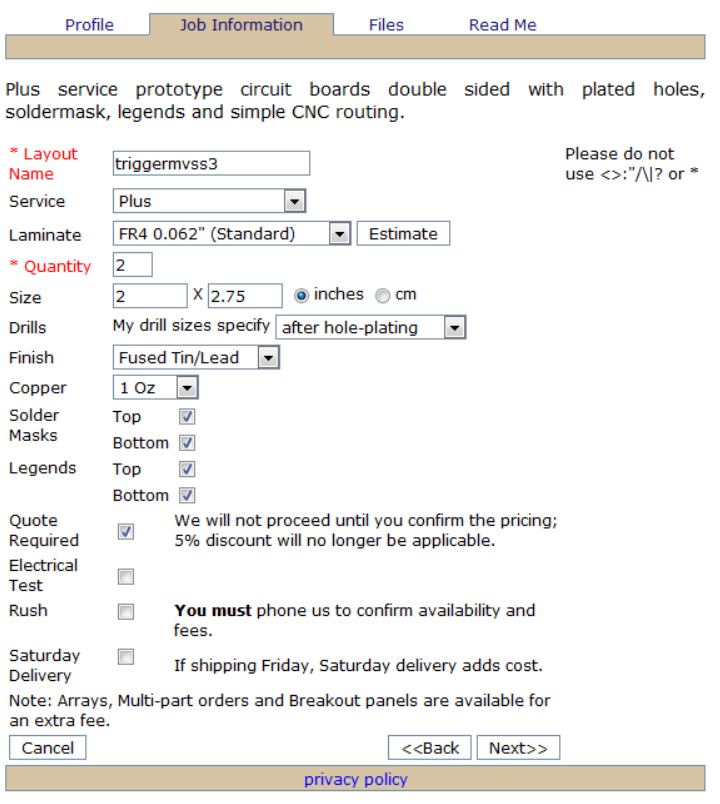
\includegraphics[scale = 0.7]{../figures/PCBorder1.PNG}
		\caption{Fill out the information as shown to generate a two sided board with silkscreen on both sides.}
		\label{fig:gerber}
	\end{figure}
	
	\begin{figure}[H]
		\centering
		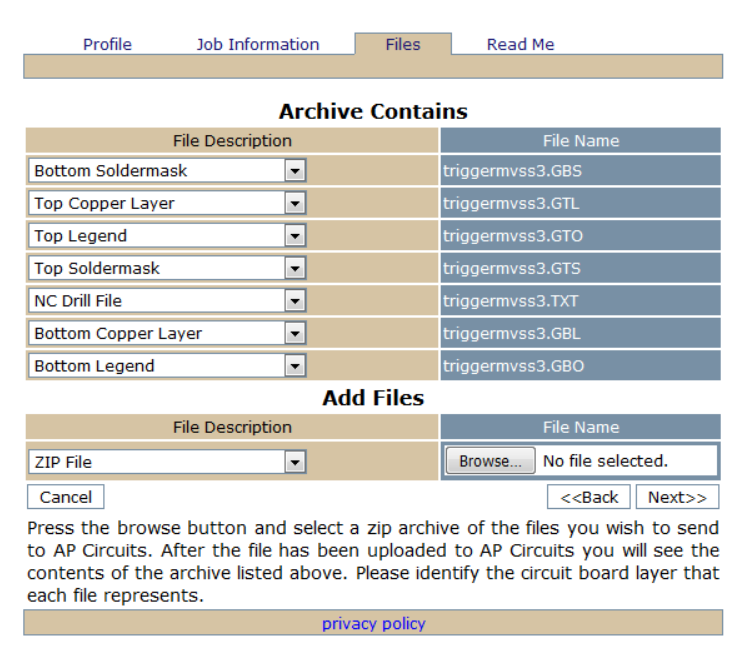
\includegraphics[scale = 0.7]{../figures/PCBorder2.PNG}
		\caption{Select the correspondences based on the file extension so that the board is manufactured correctly.}
		\label{fig:gerber}
	\end{figure}
	
	\chapter{Algorithms}
	\section{function getValue}
\label{sec:getValue}
\lstinputlisting[
caption = {The function getValue is used to parse the NMEA data to extract relevant data.},
label = {alg:getValue},
style = Matlab-editor,
basicstyle = \mlttfamily,
]{../../Matlab/getValue.m}
\cleardoublepage
\section{function calcGopro2GPStime}
\label{sec:calcGopro2GPStime}
\lstinputlisting[
caption = {The function getValue is used to parse the NMEA data to extract relevant data.},
label = {alg:getValue},
style = Matlab-editor,
basicstyle = \mlttfamily,
]{../../Matlab/calcGopro2GPStime.m}
\cleardoublepage
\section{function extractFrames}
\label{sec:extractFrames}
\lstinputlisting[
caption = {The function getValue is used to parse the NMEA data to extract relevant data.},
label = {alg:getValue},
style = Matlab-editor,
basicstyle = \mlttfamily,
]{../../Matlab/extractFrames.m}
\cleardoublepage
\section{function addPositionInfo}
\label{sec:addPositionInfo}
\lstinputlisting[
caption = {The function getValue is used to parse the NMEA data to extract relevant data.},
label = {alg:getValue},
style = Matlab-editor,
basicstyle = \mlttfamily,
]{../../Matlab/addPositionInfo.m}
\end{document}